\subsection{\texorpdfstring{模的计算 \(\operatorname{Tor}^{\mathbf{A}}(\mathbf{P},\mathbf{M})\) 与 \(\operatorname{Ext}_{\mathbf{A}}(\mathbf{M},\mathbf{N})\)}{模的计算 \textbackslash operatorname\{Tor\}\^{}\{\textbackslash mathbf\{A\}\}(\textbackslash mathbf\{P\},\textbackslash mathbf\{M\}) 与 \textbackslash operatorname\{Ext\}\_\{\textbackslash mathbf\{A\}\}(\textbackslash mathbf\{M\},\textbackslash mathbf\{N\})}}

设 M、N 为左 A-模，P 为右 A-模。此外，设 \(a: R \rightarrow M\) 是 M 的一个左分解， \(b: S \rightarrow P\) 为 P 的一个左分解，且 \(c: N \rightarrow E\) 为 N 的一个右分解。

由 X，第 49 页，命题 3 及 3 bis，存在复形态射 \(\alpha: L(M) \to R\) , \(\beta: L(P) \to S\) , \(\gamma: E \to I(N)\) 使得 \(a \circ \alpha = p_{M}\) , \(b \circ \beta = p_{P}\) , \(\gamma \circ c = e_{N}\) ；且 \(\alpha\) , \(\beta\) , \(\gamma\) 的同伦类仅依赖于给定的分解。由 X，第 64 页，命题 3 及 X，第 84 页，命题 3，态射

\[
\beta \otimes \alpha : L (P) \otimes_ {A} L (M) \rightarrow S \otimes_ {A} R,
\]

\[
\operatorname{Homgr} _ {\mathbf {A}} (\alpha , \gamma): \operatorname{Homgr} _ {\mathbf {A}} (\mathrm{R}, \mathrm{E}) \rightarrow \operatorname{Homgr} _ {\mathbf {A}} (\mathrm{L} (\mathrm{M}), \mathrm{I} (\mathrm{N}))
\]

仅依赖于给定的分解，从而通过取同调，得到次数为 0 的分次 k-同态

\[
\psi (\mathrm{S}, \mathrm{R}): \operatorname{Tor} ^ {\mathrm{A}} (\mathrm{P}, \mathrm{M}) \rightarrow \mathrm{H} (\mathrm{S} \otimes_ {\mathrm{A}} \mathrm{R}),
\]

\[
\varphi (\mathrm{R}, \mathrm{E}): \mathrm{H} \left(\operatorname{Homgr} _ {\mathrm{A}} (\mathrm{R}, \mathrm{E})\right)\rightarrow \operatorname{Ext} _ {\mathrm{A}} (\mathrm{M}, \mathrm{N}),
\]

与 α、β、γ 的选择无关。

例如，取 \(a\) , \(b\) , \(c\) 分别为 M、P、N 的恒等映射，便得到同态 \(\psi(\mathbf{P}, \mathbf{M}) : \operatorname{Tor}^{\mathbf{A}}(\mathbf{P}, \mathbf{M}) \to \mathbf{P} \otimes_{\mathbf{A}} \mathbf{M}\) 与 \(\varphi(\mathbf{M}, \mathbf{N}) : \operatorname{Hom}_{\mathbf{A}}(\mathbf{M}, \mathbf{N}) \to \operatorname{Ext}_{\mathbf{A}}(\mathbf{M}, \mathbf{N})\) 在 X，第 68 页，注记 2）以及 X，第 87 页，注记 2）中引入。

定理 1. --- a) 若分解 R 或 S 中有一个是平坦的，则 \(\psi(S, R)\) 是 \(k\) -分次模的同构。

\begin{enumerate}
\def\labelenumi{\alph{enumi})}
\setcounter{enumi}{1}
\item
  若 R 是投射的，或 E 是内射的，则 \(\varphi(\mathbf{R},\mathbf{E})\) 是 \(k\) -分次模的同构。
\item
  例如假设 R 是平坦的，并如上选择 \(\alpha\) 与 \(\beta\) 。同态 \(\beta \otimes \alpha\) 是以下态射的复合
\end{enumerate}

\[
\mathrm{L} (\mathrm{P}) \otimes_ {\mathrm{A}} \mathrm{L} (\mathrm{M}) \xrightarrow {l _ {\mathrm{L} (\mathrm{P})} \otimes \alpha} \mathrm{L} (\mathrm{P}) \otimes_ {\mathrm{A}} \mathrm{R} \xrightarrow {\beta \otimes 1 _ {\mathrm{R}}} \mathrm{S} \otimes_ {\mathrm{A}} \mathrm{R}.
\]

由于 L(P)（相应地，R）是平坦的，且 \(\alpha\) （相应地， \(\beta\) ）是同调同构，故 \(1_{L(P)} \otimes \alpha\) （相应地， \(\beta \otimes 1_R\) ）也是同调同构（X，第 67 页，命题 4）。因此 \(\beta \otimes \alpha\) 是同调同构，且 \(\psi(S, R) = H(\beta \otimes \alpha)\) 是双射。

\begin{enumerate}
\def\labelenumi{\alph{enumi})}
\setcounter{enumi}{1}
\tightlist
\item
  类似地论证，使用 X，第 86 页，命题 4。
\end{enumerate}

推论. --- 若 R 是 M 的平坦分解，则同态

\[
\psi (\mathrm{P}, \mathrm{R}): \operatorname{Tor} ^ {\mathbf {A}} (\mathrm{P}, \mathrm{M}) \rightarrow \mathrm{H} (\mathrm{P} \otimes_ {\mathbf {A}} \mathrm{R})
\]

是双射。若 R 是 M 的投射分解，则同态

\[
\varphi (\mathrm{R}, \mathrm{N}): \mathrm{H} \left(\operatorname{Homgr} _ {\mathrm{A}} (\mathrm{R}, \mathrm{N})\right)\rightarrow \operatorname{Ext} _ {\mathrm{A}} (\mathrm{M}, \mathrm{N})
\]

是双射。若 E 是 N 的内射分解，则同态

\[
\varphi (\mathbf {M}, \mathbf {E}): \mathrm{H} \left(\operatorname{Homgr} _ {\mathbf {A}} (\mathbf {M}, \mathbf {E})\right)\rightarrow \operatorname{Ext} _ {\mathbf {A}} (\mathbf {M}, \mathbf {N})
\]

是双射。

注记. --- k-模的图表

\[
\begin{array}{c} \operatorname{Tor} ^ {\mathbf {A}} (\mathrm{P}, \mathrm{M}) \xrightarrow {\psi (\mathrm{S} , \mathrm{R})} \mathrm{H} (\mathrm{S} \otimes_ {\mathbf {A}} \mathrm{R}) \\ \sigma_ {\mathrm{P}, \mathrm{M}} \Biggl \downarrow \\ \operatorname{Tor} ^ {\mathbf {A} ^ {\circ}} (\mathrm{M} ^ {\circ}, \mathrm{P} ^ {\circ}) \xrightarrow {\psi (\mathrm{R} ^ {\circ} , \mathrm{S} ^ {\circ})} \mathrm{H} (\mathrm{R} ^ {\circ} \otimes_ {\mathbf {A} ^ {\circ}} \mathrm{S} ^ {\circ}), \end{array}
\]

其中 \(\sigma_{\mathrm{P,M}}\) 与 \(\sigma(\mathrm{S},\mathrm{R})\) 是交换同构（X，第 71 页和第 63 页），该图表是交换的：实际上，它是通过取同调，由复形的交换图

\[
\begin{array}{c c} \mathrm{L} (\mathrm{P}) \otimes_ {\mathrm{A}} \mathrm{L} (\mathrm{M}) & \xrightarrow {\beta \otimes \alpha} \mathrm{S} \otimes_ {\mathrm{A}} \mathrm{R} \\ \sigma (\mathrm{L} (\mathrm{P}), \mathrm{L} (\mathrm{M})) \Big \downarrow & \Big \downarrow \sigma (\mathrm{S}, \mathrm{R}) \\ \mathrm{L} (\mathrm{M} ^ {\circ}) \otimes_ {\mathrm{A} ^ {\circ}} \mathrm{L} (\mathrm{P} ^ {\circ}) & \xrightarrow {\alpha \otimes \beta} \mathrm{R} ^ {\circ} \otimes_ {\mathrm{A} ^ {\circ}} \mathrm{S} ^ {\circ} \end{array}
\]

（“态射 \(\psi\) 与交换同构相容”）。

类似地，设 \(a_{1}: \mathbb{R}_{1} \to \mathbb{M}\) , \(b_{1}: \mathbb{S}_{1} \to \mathbb{P}\) , \(c_{1}: \mathbb{N} \to \mathbb{E}_{1}\) 为复形态射，其中 \(\mathbb{R}_{1}\) 与 \(\mathbb{S}_{1}\) 是投射的且在右侧为零，并且 \(\mathbb{E}_{1}\) 是内射的且在左侧为零。根据 X，第 49 页，命题 3 和 3 bis，存在复形态射

\[
\alpha_ {1}: \mathrm{R} _ {1} \rightarrow \mathrm{L} (\mathrm{M}), \quad \beta_ {1}: \mathrm{S} _ {1} \rightarrow \mathrm{L} (\mathrm{P}), \quad \gamma_ {1}: \mathrm{I} (\mathrm{N}) \rightarrow \mathrm{E} _ {1}
\]

使得 \(p_{\mathrm{M}} \circ \alpha_{1} = a_{1}, p_{\mathrm{P}} \circ \beta_{1} = b_{1}, \gamma_{1} \circ e_{\mathrm{N}} = c_{1}\) 由此得到复形态射

\[
\beta_ {1} \otimes \alpha_ {1}: S _ {1} \otimes_ {A} R _ {1} \rightarrow L (P) \otimes_ {A} L (M),
\]

\[
\operatorname{Homgr} _ {\mathbf {A}} \left(\alpha_ {1}, \gamma_ {1}\right): \operatorname{Homgr} _ {\mathbf {A}} \left(\mathrm{L} (\mathrm{M}), \mathrm{I} (\mathrm{N})\right)\rightarrow \operatorname{Homgr} _ {\mathbf {A}} \left(\mathrm{R} _ {1}, \mathrm{E} _ {1}\right),
\]

并且通过取同调，得到次数为 0 的 k-线性分次映射：

\[
\begin{array}{l} \psi^ {\prime} (\mathbf {S} _ {1}, \mathbf {R} _ {1}): \mathrm{H} (\mathbf {S} _ {1} \otimes_ {\mathbf {A}} \mathbf {R} _ {1}) \to \operatorname{Tor} ^ {\mathbf {A}} (\mathbf {P}, \mathbf {M}) \\ \varphi^ {\prime} (\mathbf {R} _ {1}, \mathbf {E} _ {1}): \operatorname{Ext} _ {\mathbf {A}} (\mathbf {M}, \mathbf {N}) \to \mathrm{H} (\operatorname{Homgr} _ {\mathbf {A}} (\mathbf {R} _ {1}, \mathbf {E} _ {1})) \end{array}
\]

如上所述，可验证这些映射不依赖于 \(\alpha_{1}\) , \(\beta_{1}\) , \(\gamma_{1}\) 的选择。

命题 1. --- 若 \(a_{1}\) , \(b_{1}\) , \(c_{1}\) 是同调同构，则 \(\psi^{\prime}(\mathbf{S}_{1},\mathbf{R}_{1})\) 与 \(\varphi^{\prime}(\mathbf{R}_{1},\mathbf{E}_{1})\) 分别是双射 \(\psi(\mathbf{S}_{1},\mathbf{R}_{1})\) 与 \(\varphi(\mathbf{R}_{1},\mathbf{E}_{1})\) 的逆双射。事实上， \(f = (\beta \otimes \alpha) \circ (\beta_{1} \otimes \alpha_{1})\) 是复形 \(\mathbf{S}_{1} \otimes_{\mathbf{A}} \mathbf{R}_{1}\) 到自身的态射，且有 \((b_{1} \circ \alpha_{1}) \circ f = f\) 。根据 X，第 49 页，命题 3 和 3 bis， \(f\) 是同伦等价，因此 H(f) = 1 且

\[
\psi \left(\mathrm{S} _ {1}, \mathrm{R} _ {1}\right) \circ \psi^ {\prime} \left(\mathrm{S} _ {1}, \mathrm{R} _ {1}\right) = \mathrm{H} (\beta \otimes \alpha) \circ \mathrm{H} \left(\beta_ {1} \otimes \alpha_ {1}\right) = \mathrm{H} (f) = 1;
\]

同理 \(\psi'(S_1, R_1) \circ \psi(S_1, R_1) = 1\) 。对映射 \(\varphi\) 与 \(\varphi'\) 可类似论证。

例。--- 1) 设 \(a\) 是 A 的一个元素，使得映射 \(\varphi : x \mapsto xa\) 从 A 到自身是单射（ \(a\) 不是右零因子）。利用分解

\[
0 \rightarrow \mathrm{A} _ {s} \xrightarrow {\varphi} \mathrm{A} _ {s} \rightarrow \mathrm{A} / \mathrm{A} a \rightarrow 0
\]

我们看到，对于每个右 A-模 M，有

\[
\operatorname{Tor} _ {i} ^ {\mathbf {A}} (\mathbf {M}, \mathbf {A} / \mathbf {A} a) = 0 \quad \text { for } \quad i > 1
\]

并且该 \(k\) -模 \(\operatorname{Tor}_1^{\mathbf{A}}(\mathbf{M}, \mathbf{A} / \mathbf{A}a)\) 同构于 \(\operatorname{Ker}(a_{\mathbf{M}})\) .

类似地，对于每个左 A-模 M，有

\[
\operatorname{Ext} _ {\mathbf {A}} ^ {i} (\mathbf {A} / \mathbf {A} a, \mathbf {M}) = 0 \quad \text { for } \quad i > 1
\]

且 \(k\) -模 \(\operatorname{Ext}_{\mathbf{A}}^{1}(\mathbf{A}/\mathbf{A}a, \mathbf{M})\) 同构于 \(\mathbf{M}/a\mathbf{M}\) .

\begin{enumerate}
\def\labelenumi{\arabic{enumi})}
\setcounter{enumi}{1}
\tightlist
\item
  设 A 是一个整环；令 K 为 A 的分式域，M 为一个 A-模。利用平坦分解
\end{enumerate}

\[
0 \rightarrow \mathrm{A} \rightarrow \mathrm{K} \rightarrow \mathrm{K} / \mathrm{A} \rightarrow 0
\]

（X，第 9 页，例 5），我们看到 \(\operatorname{Tor}_{i}^{\mathbf{A}}(\mathbf{K}/\mathbf{A}, \mathbf{M}) = 0\) 对 \(i > 1\) 成立；此外，考虑到 II，第 116 页，命题 26, (ii)，A-模 \(\operatorname{Tor}_{1}^{\mathbf{A}}(\mathbf{K}/\mathbf{A}, \mathbf{M})\) 同构于 M 的挠子模。

\begin{enumerate}
\def\labelenumi{\arabic{enumi})}
\setcounter{enumi}{2}
\tightlist
\item
  设 A 是一个诺特局部环，用 m 表示其极大理想，并令 \(\kappa = \mathbf{A} / \mathfrak{m}\) 。设 M 为有限生成的 A-模，P 为 M 的一个极小投射分解（X，第 54 页）。对每个 \(n \geqslant 0\) ， \(\kappa\) -向量空间 \(\operatorname{Tor}_n^{\mathbf{A}}(\kappa, \mathbf{M})\) 与 \(\operatorname{Ext}_{\mathbf{A}}^{n}(\mathbf{M}, \kappa)\) 都是有限维的，其维数等于自由 A-模 \(\mathbf{P}_n\) 的秩；事实上，复形 \(\kappa \otimes_{\mathbf{A}} \mathbf{P}\) 与 \(\operatorname{Homgr}_{\mathbf{A}}(\mathbf{P}, \kappa)\) 的微分均为零。
\end{enumerate}

\subsection{\texorpdfstring{映射的计算 \(\operatorname{Tor}^{\mathbf{A}}(g, f)\) 与 \(\operatorname{Ext}_{\mathbf{A}}(f, h)\)}{映射的计算 \textbackslash operatorname\{Tor\}\^{}\{\textbackslash mathbf\{A\}\}(g, f) 与 \textbackslash operatorname\{Ext\}\_\{\textbackslash mathbf\{A\}\}(f, h)}}

设 \(f: \mathbf{M} \to \mathbf{M}'\) , \(h: \mathbf{N}' \to \mathbf{N}\) 分别为左 A-模的同态， \(g: \mathbf{P} \to \mathbf{P}'\) 为右 A-模的同态， \(a: \mathbf{R} \to \mathbf{M}\) , \(a': \mathbf{R}' \to \mathbf{M}'\) , \(b: \mathbf{S} \to \mathbf{P}\) , \(b': \mathbf{S}' \to \mathbf{P}'\) 分别为 M、M'、P、P' 的左分解， \(c: \mathbf{N} \to \mathbf{E}\) , \(c': \mathbf{N}' \to \mathbf{E}'\) 分别为 N 与 N' 的右分解， \(\tilde{f}: \mathbf{R} \to \mathbf{R}'\) , \(\tilde{g}: \mathbf{S} \to \mathbf{S}'\) , \(\tilde{h}: \mathbf{E}' \to \mathbf{E}\) 为复形态射，使得

\[
a ^ {\prime} \circ \tilde {f} = f \circ a, b ^ {\prime} \circ \tilde {g} = g \circ b, \tilde {h} \circ c ^ {\prime} = c \circ h.
\]

命题2. --- 以下两个图表是可交换的：

\[
\begin{array}{c} \operatorname{Tor} ^ {\mathbf {A}} (\mathrm{P}, \mathrm{M}) \xrightarrow {\psi (\mathrm{S} , \mathrm{R})} \mathrm{H} (\mathrm{S} \otimes_ {\mathbf {A}} \mathrm{R}) \\ \operatorname{Tor} ^ {\mathbf {A}} (g, f) \Big \downarrow \qquad \qquad \qquad \qquad \qquad \qquad \qquad \qquad \qquad \qquad \qquad \qquad \qquad \qquad \qquad \qquad \qquad \qquad \qquad \qquad \qquad \qquad \qquad \qquad \qquad \qquad \qquad \qquad \qquad \qquad \qquad \qquad \qquad \qquad \\ \operatorname{Tor} ^ {\mathbf {A}} (\mathrm{P} ^ {\prime}, \mathrm{M} ^ {\prime}) \xrightarrow {\psi (\mathrm{S} ^ {\prime} , \mathrm{R} ^ {\prime})} \mathrm{H} (\mathrm{S} ^ {\prime} \otimes_ {\mathbf {A}} \mathrm{R} ^ {\prime})  , \end{array}
\]

\[
\begin{array}{c} \mathrm{H} (\operatorname{Homgr} _ {\mathbf {A}} (\mathrm{R} ^ {\prime}, \mathrm{E} ^ {\prime})) \xrightarrow {\varphi (\mathrm{R} ^ {\prime} , \mathrm{E} ^ {\prime})} \operatorname{Ext} _ {\mathbf {A}} (\mathrm{M} ^ {\prime}, \mathrm{N} ^ {\prime}) \\ \mathrm{H} (\operatorname{Homgr} _ {\mathbf {A}} (\tilde {f}, \tilde {h})) \Biggl \downarrow \\ \mathrm{H} (\operatorname{Homgr} _ {\mathbf {A}} (\mathrm{R}, \mathrm{E})) \xrightarrow {\varphi (\mathrm{R} , \mathrm{E})} \operatorname{Ext} _ {\mathbf {A}} (\mathrm{M}, \mathrm{N}). \end{array}
\]

设 \(\alpha: L(M) \to R\) , \(\alpha': L(M') \to R'\) , \(\gamma: L(P) \to S\) , \(\gamma': L(P') \to S'\) 为复形态射，使得

\[
a \circ \alpha = p _ {\mathrm{M}}, a ^ {\prime} \circ \alpha^ {\prime} = p _ {\mathrm {M^ {\prime}}}, b \circ \gamma = p _ {\mathrm{P}}, b ^ {\prime} \circ \gamma^ {\prime} = p _ {\mathrm {P^ {\prime}}}.
\]

根据定义， \(\mathrm{H}(\tilde{g}\otimes\tilde{f})\circ\psi(\mathrm{S},\mathrm{R})\) 等于

\[
\mathrm{H} (\tilde {g} \otimes \tilde {f}) \circ \mathrm{H} (\gamma \otimes \alpha) = \mathrm{H} ((\tilde {g} \circ \gamma) \otimes (\tilde {f} \circ \alpha)),
\]

而 \(\psi(\mathbf{S}',\mathbf{R}')\circ\mathrm{Tor}^{\mathbf{A}}(g,f)\) 等于

\[
\mathrm{H} \left(\gamma^ {\prime} \otimes \alpha^ {\prime}\right) \circ \mathrm{H} \left(\mathrm{L} (g) \otimes \mathrm{L} (f)\right) = \mathrm{H} \left(\left(\gamma^ {\prime} \circ \mathrm{L} (g)\right) \otimes \left(\alpha^ {\prime} \circ \mathrm{L} (f)\right)\right).
\]

另一方面， \(\alpha' \circ L(f)\) 与 \(\tilde{f} \circ \alpha\) 是从 L(M) 到 R′ 的两个态射，使得 \(a' \circ (\alpha' \circ L(f)) = p_{\mathrm{M}} \circ L(f) = f \circ p_{\mathrm{M}} = f \circ a \circ \alpha = a' \circ (\tilde{f} \circ \alpha)\) 。根据 X，第 49 页，命题 3， \(\alpha' \circ L(f)\) 与 \(\tilde{f} \circ \alpha\) 是同伦的；同样地 \(\gamma' \circ L(g)\) 与 \(\tilde{g} \circ \gamma\) 是同伦的，因此 \((\gamma' \circ L(g)) \otimes (\alpha' \circ L(f))\) 与 \((\tilde{g} \circ \gamma) \otimes (\tilde{f} \circ \alpha)\) 根据 X，第 64 页，命题 3 也是同伦的。因此我们有

\[
\begin{array}{r l} \mathrm{H} (\tilde {g} \otimes \tilde {f}) \circ \psi (\mathrm{S}, \mathrm{R}) & = \mathrm{H} ((\tilde {g} \circ \gamma) \otimes (\tilde {f} \circ \alpha)) = \mathrm{H} ((\gamma^ {\prime} \circ \mathrm{L} (g)) \otimes (\alpha^ {\prime} \circ \mathrm{L} (f))) \\ & = \psi (\mathrm{S} ^ {\prime}, \mathrm{R} ^ {\prime}) \circ \mathrm{Tor} ^ {\mathrm{A}} (g, f). \end{array}
\]

我们类似地论证第二个图表。

注记. --- 类似地考虑复形态射的交换图表。

\[
\begin{array}{c c c} \mathrm{R} _ {1} \xrightarrow {a _ {1}} \mathrm{M} & \mathrm{S} _ {1} \xrightarrow {b _ {1}} \mathrm{P} & \mathrm{N} ^ {\prime} \xrightarrow {c _ {1} ^ {\prime}} \mathrm{E} ^ {\prime} \\ \tilde {f} \Big \downarrow & f \Big \downarrow & g \Big \downarrow \\ \mathrm{R} _ {1} ^ {\prime} \xrightarrow {a _ {1} ^ {\prime}} \mathrm{M} ^ {\prime} & \mathrm{S} _ {1} ^ {\prime} \xrightarrow {b _ {1} ^ {\prime}} \mathrm{P} ^ {\prime} & \mathrm{N} \xrightarrow {c _ {1}} \mathrm{E} _ {1} \end{array}
\]

其中复形 \(R_{1}\) , \(R_{1}^{\prime}\) , \(S_{1}\) , \(S_{1}^{\prime}\) 是投射的且在右侧为零，而复形 \(E_{1}\) , \(E_{1}^{\prime}\) 是内射的且在左侧为零。那么

\[
\begin{array}{r l} & {\mathrm{Tor} ^ {\mathbf {A}} (g, f) \circ \psi^ {\prime} (\mathrm{S} _ {1}, \mathrm{R} _ {1}) = \psi^ {\prime} (\mathrm{S} _ {1} ^ {\prime}, \mathrm{R} _ {1} ^ {\prime}) \circ \mathrm{H} (\tilde {g} \otimes \tilde {f})} \\ & {\varphi^ {\prime} (\mathrm{R} _ {1}, \mathrm{E} _ {1}) \circ \mathrm{Ext} _ {\mathbf {A}} (f, h) = \mathrm{H} (\mathrm{Homgr} _ {\mathbf {A}} (\tilde {f}, \tilde {h})) \circ \varphi^ {\prime} (\mathrm{R} _ {1} ^ {\prime}, \mathrm{E} _ {1} ^ {\prime})} \end{array}
\]

这由与命题 2 类似的论证得到。

\subsection{连接同态的计算}

考虑一个交换图

\begin{enumerate}
\def\labelenumi{(\arabic{enumi})}
\tightlist
\item
\end{enumerate}

\[
\begin{array}{c} 0 \longrightarrow \mathrm{R} ^ {\prime} \xrightarrow {\tilde {u}} \mathrm{R} \xrightarrow {\tilde {v}} \mathrm{R} ^ {\prime \prime} \longrightarrow 0 \\ a ^ {\prime} \Big \downarrow \qquad \qquad \qquad \qquad \qquad \qquad \qquad \qquad \qquad \qquad \qquad \qquad \qquad \qquad \qquad \qquad \qquad \qquad \qquad \qquad \qquad \qquad \qquad \qquad \qquad \qquad \qquad \qquad \qquad \qquad \qquad \qquad \qquad \qquad \\ 0 \longrightarrow \mathrm{M} ^ {\prime} \xrightarrow {u} \mathrm{M} \xrightarrow {v} \mathrm{M} ^ {\prime \prime} \longrightarrow 0 \end{array}\tag{2}
\]

其中第一行 (1) 是左 A-模复形的正合列，第二行 (2) 是左 A-模的正合列，且竖直箭头为左分解。

命题 3. --- a) 设 P 是一个 A-模， \(b: S \to P\) 为 P 的一个左分解；假设 k-模复形序列

\[
0 \rightarrow \mathrm{S} \otimes_ {\mathrm{A}} \mathrm{R} ^ {\prime} \xrightarrow {l _ {\mathrm{s}} \otimes \tilde {u}} \mathrm{S} \otimes_ {\mathrm{A}} \mathrm{R} \xrightarrow {l _ {\mathrm{s}} \otimes \tilde {v}} \mathrm{S} \otimes_ {\mathrm{A}} \mathrm{R} ^ {\prime \prime} \rightarrow 0\tag{3}
\]

是正合的。则下面的图表是交换的：

\[
\begin{array}{c c c} \operatorname{Tor} ^ {\mathbf {A}} (\mathrm{P}, \mathrm{M} ^ {\prime \prime}) & \xrightarrow {\partial (\mathrm{P} , (2))} & \operatorname{Tor} ^ {\mathbf {A}} (\mathrm{P}, \mathrm{M} ^ {\prime}) \\ \psi (\mathrm{S}, \mathrm{R} ^ {\prime \prime}) \Big \downarrow & & \Big \downarrow \psi (\mathrm{S}, \mathrm{R} ^ {\prime}) \\ \mathrm{H} (\mathrm{S} \otimes_ {\mathbf {A}} \mathrm{R} ^ {\prime \prime}) & \xrightarrow {\partial ((3))} & \mathrm{H} (\mathrm{S} \otimes_ {\mathbf {A}} \mathrm{R} ^ {\prime}). \end{array}
\]

\begin{enumerate}
\def\labelenumi{\alph{enumi})}
\setcounter{enumi}{1}
\tightlist
\item
  设 N 是一个左 A-模， \(c : N \to E\) 为 N 的一个右分解；假设 k-模复形序列
\end{enumerate}

\begin{enumerate}
\def\labelenumi{(\arabic{enumi})}
\setcounter{enumi}{3}
\tightlist
\item
\end{enumerate}

\(0 \to \text{Homgr}_{\mathbf{A}}(\mathbf{R}^{\prime \prime}, \mathbf{E}) \xrightarrow{\text{Homgr}_{\mathbf{A}}(\tilde{\imath}, 1)} \text{Homgr}_{\mathbf{A}}(\mathbf{R}, \mathbf{E}) \xrightarrow{\text{Homgr}_{\mathbf{A}}(\tilde{\mu}, 1)} \text{Homgr}_{\mathbf{A}}(\mathbf{R}^{\prime}, \mathbf{E}) \to 0\) 是正合的。则下面的图表是交换的：

\[
\begin{array}{c} \mathrm{H} (\operatorname{Homgr} _ {\mathbf {A}} (\mathrm{R} ^ {\prime}, \mathrm{E})) \xrightarrow {\delta ((4))} \mathrm{H} (\operatorname{Homgr} _ {\mathbf {A}} (\mathrm{R} ^ {\prime \prime}, \mathrm{E})) \\ \varphi (\mathrm{R} ^ {\prime}, \mathrm{E}) \Big \downarrow \\ \operatorname{Ext} _ {\mathbf {A}} (\mathrm{M} ^ {\prime}, \mathrm{N}) \xrightarrow {\partial ((2) , \mathrm{N})} \operatorname{Ext} _ {\mathbf {A}} (\mathrm{M} ^ {\prime \prime}, \mathrm{N}). \end{array}
\]

例如证明 \(a\) )。设 \(\beta: L(P) \to S\) 是复形的态射，使得 \(b \circ \beta = p_{P}\) ；考虑 \(k\) -复形的图表

\[
\begin{array}{c}0 \rightarrow \mathrm{S} \otimes_ {\mathrm{A}} \mathrm{R} ^ {\prime} \xrightarrow {1 \otimes \tilde {u}} \mathrm{S} \otimes_ {\mathrm{A}} \mathrm{R} \xrightarrow {1 \otimes \tilde {v}} \mathrm{S} \otimes_ {\mathrm{A}} \mathrm{R} ^ {\prime \prime} \longrightarrow 0\\\beta \otimes 1 _ {\mathrm{R}} \Bigg | \quad \beta \otimes 1 _ {\mathrm{R}} \Bigg | \quad \beta \otimes 1 _ {\mathrm{R}} \Bigg |\\0 \rightarrow \mathrm{L(P)} \otimes_ {\mathrm{A}} \mathrm{R} ^ {\prime} \xrightarrow {1 \otimes \tilde {u}} \mathrm{L(P)} \otimes_ {\mathrm{A}} \mathrm{R} \xrightarrow {1 \otimes \tilde {v}} \mathrm{L(P)} \otimes_ {\mathrm{A}} \mathrm{R} ^ {\prime \prime} \longrightarrow 0\\1 \otimes a ^ {\prime} \Bigg | \quad 1 \otimes a \Bigg | \quad 1 \otimes a ^ {\prime \prime} \Bigg |\\0 \rightarrow \mathrm{L(P)} \otimes_ {\mathrm{A}} \mathrm{M} ^ {\prime} \xrightarrow {1 \otimes u} \mathrm{L(P)} \otimes_ {\mathrm{A}} \mathrm{M} \xrightarrow {1 \otimes v} \mathrm{L(P)} \otimes_ {\mathrm{A}} \mathrm{M} ^ {\prime \prime} \longrightarrow 0.\end{array}
\]

它是交换的且各行正合（第一行由假设，另外两行由 L(P) 是平坦的这一事实）。因此我们有交换图（X，第 31 页，命题 2，以及 X，第 72 页，定义 2）。

\[
\begin{array}{c c c} \mathrm{H} (\mathrm{S} \otimes_ {\mathrm{A}} \mathrm{R} ^ {\prime \prime}) & \xrightarrow {\partial ((3))} & \mathrm{H} (\mathrm{S} \otimes_ {\mathrm{A}} \mathrm{R} ^ {\prime}) \\ \mathrm{H} (\beta \otimes 1) \uparrow & & \uparrow \mathrm{H} (\beta \otimes 1) \\ \mathrm{H} (\mathrm{L} (\mathrm{P}) \otimes_ {\mathrm{A}} \mathrm{R} ^ {\prime \prime}) & \longrightarrow & \mathrm{H} (\mathrm{L} (\mathrm{P}) \otimes_ {\mathrm{A}} \mathrm{R} ^ {\prime}) \\ \mathrm{H} (1 \otimes a ^ {\prime \prime}) \downarrow & & \downarrow \mathrm{H} (1 \otimes a ^ {\prime}) \\ \mathrm{H} (\mathrm{L} (\mathrm{P}) \otimes_ {\mathrm{A}} \mathrm{M} ^ {\prime \prime}) & \longrightarrow & \mathrm{H} (\mathrm{L} (\mathrm{P}) \otimes_ {\mathrm{A}} \mathrm{M} ^ {\prime}) \\ \psi_ {\mathrm{P}} (\mathbf {M} ^ {\prime \prime}) \uparrow & & \uparrow \psi_ {\mathrm{P}} (\mathbf {M} ^ {\prime}) \\ \operatorname{Tor} (\mathrm{P}, \mathbf {M} ^ {\prime \prime}) & \xrightarrow {\partial (\mathrm{P} , (2))} & \operatorname{Tor} (\mathrm{P}, \mathbf {M} ^ {\prime}). \end{array}
\]

由 X，第 67 页，命题 4，H(1 ⊗ a′′) 和 H(1 ⊗ a′) 是双射；另一方面，根据同态 ψ 的定义，我们有 H(β ⊗ 1) ∘ ψ(L(P), R′′) = ψ(S, R′′) 以及 H(1 ⊗ a′′)∘ψ(L(P), R′′) = ψ(L(P), M′′) = ψ\_P(M′′)，因此

\[
\psi (\mathrm{S}, \mathrm{R} ^ {\prime \prime}) = \mathrm{H} (\beta \otimes 1) \circ \mathrm{H} (1 \otimes a ^ {\prime \prime}) ^ {- 1} \circ \psi_ {\mathrm{P}} (\mathrm{M} ^ {\prime \prime});
\]

类似地， \(\psi(S, R') = H(\beta \otimes 1) \circ H(1 \otimes a')^{-1} \circ \psi_P(M')\) ，而所需的结论 \(\partial((3)) \circ \psi(S, R'') = \psi(S, R') \circ \partial(P, (2))\) 由上面图表的交换性得出。

注记. --- 1) 利用交换同构，由 a) 可推出将张量积的两个变元互换角色后所得的类似命题。

\begin{enumerate}
\def\labelenumi{\arabic{enumi})}
\setcounter{enumi}{1}
\tightlist
\item
  沿用 \(a\) ) 的记号，假设 S 平坦，或 R、R'、R'' 平坦；则一方面序列 (3) 是正合的（X，第 72 页，推论 2），从而可应用命题 3；另一方面 \(\psi(S, R')\) 是双射的（定理 1），因此
\end{enumerate}

\[
\partial (\mathrm{P}, (2)) = \psi (\mathrm{S}, \mathrm{R} ^ {\prime}) ^ {- 1} \circ \partial ((3)) \circ \psi (\mathrm{S}, \mathrm{R} ^ {\prime \prime}).
\]

\begin{enumerate}
\def\labelenumi{\arabic{enumi})}
\setcounter{enumi}{2}
\tightlist
\item
  沿用 \(b\) ) 的记号，假设 E 是内射的，或者 R、R'、R'\,' 是投射的；则一方面序列 (4) 是正合的（X，第 83 页，命题 2），可以应用命题 3；另一方面， \(\varphi(R', E)\) 是双射的（定理 1）；因此
\end{enumerate}

\[
\delta ((2), \mathrm{N}) = \varphi (\mathrm{R} ^ {\prime \prime}, \mathrm{E}) \circ \hat {\partial} ((4)) \circ \varphi (\mathrm{R} ^ {\prime}, \mathrm{E}) ^ {- 1}.
\]

现在考虑一个交换图，其第一行 (5) 是左 A-模的正合列，第二行 (6) 是左 A-模复形的正合列，且竖直箭头是右分解。如同命题 3 中的推理，可证明以下命题：

\begin{enumerate}
\def\labelenumi{(\arabic{enumi})}
\setcounter{enumi}{4}
\tightlist
\item
\end{enumerate}

\[
\begin{array}{c} 0 \longrightarrow \mathrm{N} ^ {\prime} \xrightarrow {r} \mathrm{N} \xrightarrow {s} \mathrm{N} ^ {\prime \prime} \longrightarrow 0 \\ c ^ {\prime} \Big \downarrow \qquad \qquad c \Big \downarrow \qquad \qquad c ^ {\prime \prime} \Big \downarrow \\ 0 \longrightarrow \mathrm{E} ^ {\prime} \xrightarrow {\tilde {r}} \mathrm{E} \xrightarrow {\tilde {s}} \mathrm{E} ^ {\prime \prime} \longrightarrow 0 \end{array}\tag{6}
\]

命题 4. --- 设 M 是左 A-模，

且 \(a: \mathbf{R} \to \mathbf{M}\) 为 M 的一个左分解，使得序列

\begin{enumerate}
\def\labelenumi{(\arabic{enumi})}
\setcounter{enumi}{6}
\tightlist
\item
  \(0 \to \operatorname{Homgr}_{\mathbf{A}}(\mathbf{R}, \mathbf{E}') \xrightarrow{\operatorname{Homgr}(\tilde{\mathcal{S}}, 1)} \operatorname{Homgr}_{\mathbf{A}}(\mathbf{R}, \mathbf{E}) \xrightarrow{\operatorname{Homgr}(\tilde{\mathcal{F}}, 1)} \operatorname{Homgr}_{\mathbf{A}}(\mathbf{R}, \mathbf{E}'' \to 0\) 是正合的。则下图是交换的。
\end{enumerate}

\[
\begin{array}{c} \mathrm{H} (\operatorname{Homgr} _ {\mathbf {A}} (\mathbf {R}, \mathbf {E} ^ {\prime \prime})) \xrightarrow {\partial ((7))} \mathrm{H} (\operatorname{Homgr} _ {\mathbf {A}} (\mathbf {R}, \mathbf {E} ^ {\prime})) \\ \varphi (\mathbf {R}, \mathbf {E} ^ {\prime \prime}) \Biggl \downarrow \\ \operatorname{Ext} _ {\mathbf {A}} (\mathbf {M}, \mathbf {N} ^ {\prime \prime}) \xrightarrow {\delta (\mathbf {M} , (5))} \operatorname{Ext} _ {\mathbf {A}} (\mathbf {M}, \mathbf {N} ^ {\prime}). \end{array}
\]

注记. --- 4) 若 R 是投射的，或 E、E'、E'' 是内射的，则序列 (7) 是正合的（X，第 83 页，命题 2）；此外，φ(R, E'') 是双射的（定理 1）；因此

\[
\delta (M, (5)) = \varphi (R, E ^ {\prime}) \circ \partial ((7)) \circ \varphi (R, E ^ {\prime \prime}) ^ {- 1}.
\]

\begin{enumerate}
\def\labelenumi{\arabic{enumi})}
\setcounter{enumi}{4}
\tightlist
\item
  我们把与命题 3 和命题 4 类似且关于同态 \(\psi_{1}\) 与 \(\varphi_{1}\) 的命题的陈述与证明留给读者。
\end{enumerate}

\subsection{扩张模与挠模的有限性}

设 M 是左 A-模，I 是滤过预序集， \((\mathbf{N}_{i}, u_{ji})\) 是关于 I 的左 A-模归纳系， \(N = \varinjlim N_{i}\) 为其归纳极限， \(u_{i}: N_{i} \to N, i \in I\) 为典范映射。则 \((\operatorname{Ext}_{\mathbf{A}}(\mathbf{M}, \mathbf{N}_{i}), \operatorname{Ext}_{\mathbf{A}}(1_{\mathbf{M}}, u_{ji}))\) 是 k-模的归纳系， \((\operatorname{Ext}_{\mathbf{A}}(1_{\mathbf{M}}, u_{i}))\) 是映射的归纳系，其归纳极限是分次 k-模的同态，称为典范同态

\[
\varinjlim_ {i \in I} \operatorname{Ext} _ {\mathbf {A}} (\mathbf {M}, \mathbf {N} _ {i}) \rightarrow \operatorname{Ext} _ {\mathbf {A}} \left(\mathbf {M}, \varinjlim_ {i \in I} \mathbf {N} _ {i}\right).\tag{8}
\]

命题 5. --- 若 A 是左诺特的且 M 是有限生成 A-模，则典范同态 (8) 是双射的。

事实上，设（X，第 53 页，命题 6）\(p: L \to M\) 为 M 的自由分解，使得 \(L_{n}\) 对每个 \(n\) 都是有限生成的。从 \(k\) -复形

\[
u: \varinjlim \operatorname{Homgr} _ {\mathbf {A}} (\mathrm{L}, \mathrm{N} _ {i}) \rightarrow \operatorname{Homgr} _ {\mathbf {A}} (\mathrm{L}, \varinjlim \mathrm{N} _ {i})
\]

是双射的，因此同态

\[
\varinjlim \mathrm{H} (\operatorname{Homgr} _ {\mathrm{A}} (\mathrm{L}, \mathrm{N} _ {i})) \rightarrow \mathrm{H} (\operatorname{Homgr} _ {\mathrm{A}} (\mathrm{L}, \varinjlim \mathrm{N} _ {i}))
\]

推出同态 \(\mathrm{H}(\mathrm{Homgr}(1,u_{i}))\) （X，第 28 页，命题 1）。然后由命题 2（X，第 103 页）和定理 1（X，第 100 页）得出结论。

命题 6. --- 设 B 是环，N 是 (A, B)-双模，且为诺特 B-模（相应地，有限长度）。

\begin{enumerate}
\def\labelenumi{\alph{enumi})}
\item
  假设 A 是右诺特的，设 M 是有限生成右 A-模。则 B-模（X，第 81 页）Tor \(_{n}^{A}\) (M, N) 是诺特的（相应地，有限长度的）。
\item
  假设 A 是左诺特的，设 M 是有限生成左 A-模。则 B-模（X，第 98 页）Ext \(_{A}^{n}\) (M, N) 是诺特的（相应地，有限长度的）。
\end{enumerate}

选取自由分解 \(p: \mathbf{L} \to \mathbf{M}\) ，使得每个 A-模 \(\mathbf{L}_n\) 都是有限生成的（X，第 53 页，命题 6），并设 C 为 B-模复形 \(\mathbf{L} \otimes_{\mathbf{A}} \mathbf{N}\) （情形 \(a\) )）或 \(\operatorname{Homgr}_{\mathbf{A}}(\mathbf{L}, \mathbf{N})\) （情形 \(b\) )）。每个 B-模 \(\mathbf{C}_n\) 同构于 N 的有限个拷贝的乘积，因此是诺特的（相应地，有限长度的）；从而模 \(\mathrm{H}_n(\mathbf{C})\) 亦然。现在，根据 X，第 100 页，定理 1，这些模同构于 \(\operatorname{Tor}_n^{\mathbf{A}}(\mathbf{M}, \mathbf{N})\) （情形 \(a\) )）或 \(\operatorname{Ext}_{\mathbf{A}}^{-n}(\mathbf{M}, \mathbf{N})\) （情形 \(b\) )）。

推论. --- 设 \(\rho: A \to B\) 为诺特交换环的同态，M 为有限生成 A-模，N 为 B-模。若 N 是有限生成（相应地，有限长度）B-模，则 B-模 \(\operatorname{Tor}_{n}^{A}(M, N)\) 与 \(\operatorname{Ext}_{A}^{n}(M, N)\) 也是。

\subsection{\texorpdfstring{同态 \(\operatorname{Tor}^{\mathbf{B}}(\mathbf{P},\mathbf{N})\otimes_{\mathbf{A}}\mathbf{Q}\to \operatorname{Tor}^{\mathbf{B}}(\mathbf{P},\mathbf{N}\otimes_{\mathbf{A}}\mathbf{Q})\) 与 \(\operatorname{Ext}_{\mathbf{B}}(\mathbf{M},\mathbf{N})\otimes_{\mathbf{A}}\mathbf{Q}\rightarrow \operatorname{Ext}_{\mathbf{B}}(\mathbf{M},\mathbf{N}\otimes_{\mathbf{A}}\mathbf{Q})\)}{张量积下的 Tor 与 Ext 同态}}

设 B 是环，N 是 (B, A)-双模，M 是左 B-模，P 是右 B-模，Q 是左 A-模。

根据 X，第 62 页，我们有同态

\[
\gamma_ {1}: \mathrm{H} (\mathrm{L} (\mathrm{P}) \otimes_ {\mathrm{B}} \mathrm{N}) \otimes_ {\mathrm{A}} \mathrm{Q} \rightarrow \mathrm{H} (\mathrm{L} (\mathrm{P}) \otimes_ {\mathrm{B}} \mathrm{N} \otimes_ {\mathrm{A}} \mathrm{Q});
\]

此外（X，第 69 页，命题 5），我们有同构

\[
\begin{array}{c} \psi_ {1} (N): \operatorname{Tor} ^ {B} (P, N) \otimes_ {A} Q \qquad H (L (P) \otimes_ {B} N) \otimes_ {A} Q, \\ \psi_ {1} (N \otimes_ {A} Q): \operatorname{Tor} ^ {B} (P, N \otimes_ {A} Q) \to H (L (P) \otimes_ {B} N \otimes_ {A} Q). \end{array}
\]

典范的 0 次分次同态

\[
\operatorname{Tor} ^ {\mathrm{B}} (\mathrm{P}, \mathrm{N}) \otimes_ {\mathrm{A}} \mathrm{Q} \rightarrow \operatorname{Tor} ^ {\mathrm{B}} (\mathrm{P}, \mathrm{N} \otimes_ {\mathrm{A}} \mathrm{Q})\tag{9}
\]

定义为复合 \(\psi_{\mathrm{P}}(\mathbf{N}\otimes_{\mathbf{A}}\mathbf{Q})^{-1}\circ \gamma_{1}\circ (\psi_{\mathrm{P}}(\mathbf{N})\otimes 1_{\mathbf{Q}})\) .

类似地，由复形的典范态射

\[
\alpha : \operatorname{Homgr} _ {B} (L (M), N) \otimes_ {A} Q \rightarrow \operatorname{Homgr} _ {B} (L (M), N \otimes_ {A} Q)
\]

由此推出同态 H(α)；我们有典范同态（X，第 62 页）

\[
\gamma_ {2}: \mathrm{H} (\operatorname{Homgr} _ {\mathrm{B}} (L (M), N)) \otimes_ {A} Q \rightarrow \mathrm{H} (\operatorname{Homgr} _ {\mathrm{B}} (L (M), N) \otimes_ {A} Q),
\]

和同构（X，第 88 页，命题 5）

\[
\begin{array}{c} \varphi_ {\mathrm{M}} (\mathrm{N}): \mathrm{H} \big (\operatorname{Homgr} _ {\mathrm{B}} (\mathrm{L} (\mathrm{M}), \mathrm{N}) \big) \otimes_ {\mathrm{A}} \mathrm{Q} \to \operatorname{Ext} _ {\mathrm{B}} (\mathrm{M}, \mathrm{N}) \otimes_ {\mathrm{A}} \mathrm{Q}, \\ \varphi_ {\mathrm{M}} (\mathrm{N} \otimes_ {\mathrm{A}} \mathrm{Q}): \mathrm{H} \big (\operatorname{Homgr} _ {\mathrm{B}} (\mathrm{L} (\mathrm{M}), \mathrm{N} \otimes_ {\mathrm{A}} \mathrm{Q}) \big) \to \operatorname{Ext} _ {\mathrm{B}} (\mathrm{M}, \mathrm{N} \otimes_ {\mathrm{A}} \mathrm{Q}). \end{array}
\]

典范的 0 次分次同态

\[
\operatorname{Ext} _ {\mathbf {B}} (\mathbf {M}, \mathbf {N}) \otimes_ {\mathbf {A}} \mathbf {Q} \rightarrow \operatorname{Ext} _ {\mathbf {B}} (\mathbf {M}, \mathbf {N} \otimes_ {\mathbf {A}} \mathbf {Q})\tag{10}
\]

定义为复合

\[
\varphi_ {\mathrm{M}} (\mathrm{N} \otimes_ {\mathrm{A}} \mathrm{Q}) \circ \mathrm{H} (\alpha) \circ \gamma_ {2} \circ \left(\varphi_ {\mathrm{M}} (\mathrm{N}) \otimes 1 _ {\mathrm{Q}}\right) ^ {- 1}.
\]

命题 7. --- a) 若 A-模 Q 是平坦的，则同态 (9) 是双射的。b) 若 A-模 Q 是有限生成投射的，则同态 (10) 是双射的。

\begin{enumerate}
\def\labelenumi{\alph{enumi})}
\setcounter{enumi}{2}
\item
  若 A-模 Q 是平坦的，环 B 是诺特的，且 B-模 M 是有限生成的，则同态 (10) 是双射的。
\item
  若 Q 是平坦的， \(\gamma_{1}\) 是双射的（X，第 66 页，推论 2）。
\item
  若 Q 是有限生成投射的，则它是平坦的，因此 \(\gamma_{2}\) 是双射的，而且 \(\alpha\) 是双射的（II，第 75 页，命题 2，a)）。
\item
  在 c) 的假设下， \(\gamma_{2}\) 是双射的，因为 Q 是平坦的。此外（X，第 53 页，命题 6），存在 M 的分解 L，使得每个 \(\mathbf{L}_{n}\) 都是有限生成自由的；设 \(u: \mathbf{L}(\mathbf{M}) \to \mathbf{L}\) 是同伦等价（X，第 49 页，命题 3 的推论）；在交换图中，
\end{enumerate}

\[
\begin{array}{c c c} \operatorname{Homgr} _ {\mathrm{B}} (\mathrm{L} (\mathrm{M}), \mathrm{N}) \otimes_ {\mathrm{A}} \mathrm{Q} & \xrightarrow {\alpha} & \operatorname{Homgr} _ {\mathrm{B}} (\mathrm{L} (\mathrm{M}), \mathrm{N} \otimes_ {\mathrm{A}} \mathrm{Q}) \\ \uparrow & & \uparrow \\ \operatorname{Homgr} _ {\mathrm{B}} (\mathrm{L}, \mathrm{N}) \otimes_ {\mathrm{A}} \mathrm{Q} & \xrightarrow {\bar {\alpha}} & \operatorname{Homgr} _ {\mathrm{B}} (\mathrm{L}, \mathrm{N} \otimes_ {\mathrm{A}} \mathrm{Q}). \end{array}
\]

由 \(u\) 推出的竖直箭头是同伦等价（X，第 64 页，命题 3 和第 83 页，命题 3），且 \(\overline{\alpha}\) 是双射的（II，第 75 页，命题 2 (ii)）；因此 H(α) 是双射的，且同态 (10) 是双射的。

\subsection{\texorpdfstring{同态 \(\operatorname{Tor}^{\mathbf{B}}(\mathbf{P},\mathbf{N}\otimes_{\mathbf{A}}\mathbf{Q})\to \operatorname{Tor}^{\mathbf{A}}(\mathbf{P}\otimes_{\mathbf{B}}\mathbf{N},\mathbf{Q})\) 与 \(\operatorname{Ext}_{\mathbf{A}}(\mathbf{Q},\operatorname{Hom}_{\mathbf{B}}(\mathbf{N},\mathbf{M}))\to \operatorname{Ext}_{\mathbf{B}}(\mathbf{N}\otimes_{\mathbf{A}}\mathbf{Q},\mathbf{M})\)}{Tor 与 Ext 的换环同态}}

沿用前面的记号，并假设 N 在 A 上是平坦的。则态射 \(\mathrm{N}\otimes_{\mathbf{A}}\mathrm{L}(\mathrm{Q})\xrightarrow{\mathrm{1}\otimes p_{\mathrm{Q}}} \mathrm{N}\otimes_{\mathbf{A}}\mathrm{Q}\) 是一个拟同构（X，第 67 页，命题 4），因此同态

\[
\psi (\mathrm{P}, \mathrm{N} \otimes_ {\mathrm{A}} \mathrm{L} (\mathrm{Q})): \operatorname{Tor} ^ {\mathrm{B}} (\mathrm{P}, \mathrm{N} \otimes_ {\mathrm{A}} \mathrm{Q}) \rightarrow \mathrm{H} (\mathrm{P} \otimes_ {\mathrm{B}} \mathrm{N} \otimes_ {\mathrm{A}} \mathrm{L} (\mathrm{Q}))
\]

\[
\varphi (\mathrm{N} \otimes_ {\mathrm{A}} \mathrm{L} (\mathrm{Q}), \mathrm{M}): \mathrm{H} (\operatorname{Homgr} _ {\mathrm{B}} (\mathrm{N} \otimes_ {\mathrm{A}} \mathrm{L} (\mathrm{Q}), \mathrm{M})) \rightarrow \operatorname{Ext} _ {\mathrm{B}} (\mathrm{N} \otimes_ {\mathrm{A}} \mathrm{Q}, \mathrm{M}).
\]

再利用同构

\[
\begin{array}{c} \overline {{\psi}} _ {Q} (P \otimes_ {B} N): \operatorname{Tor} ^ {A} (P \otimes_ {B} N, Q) \to H (P \otimes_ {B} N \otimes_ {A} L (Q)), \\ \beta : \operatorname{Homgr} _ {A} (L (Q), \operatorname{Hom} _ {B} (N, M)) \to \operatorname{Homgr} _ {B} (N \otimes_ {A} L (Q), M), \\ \varphi_ {Q} (\operatorname{Hom} _ {B} (N, M)): H (\operatorname{Homgr} _ {A} (L (Q), \operatorname{Hom} _ {B} (N, M))) \to \operatorname{Ext} _ {A} (Q, \operatorname{Hom} _ {B} (N, M)), \end{array}
\]

由此，我们推出次数为 0 的典范分次同态：

\begin{enumerate}
\def\labelenumi{(\arabic{enumi})}
\setcounter{enumi}{10}
\tightlist
\item
\end{enumerate}

\[
\operatorname{Tor} ^ {\mathbf {B}} (\mathrm{P}, \mathrm{N} \otimes_ {\mathrm{A}} \mathrm{Q}) \rightarrow \operatorname{Tor} ^ {\mathbf {A}} (\mathrm{P} \otimes_ {\mathrm{B}} \mathrm{N}, \mathrm{Q})\tag{12}
\]

\[
\operatorname{Ext} _ {\mathbf {A}} \left(\mathrm{Q}, \operatorname{Hom} _ {\mathbf {B}} (\mathrm{N}, \mathrm{M})\right)\rightarrow \operatorname{Ext} _ {\mathbf {B}} \left(\mathrm{N} \otimes_ {\mathbf {A}} \mathrm{Q}, \mathrm{M}\right).
\]

命题 8. --- a) 若 N 在 A 上和 B 上都是平坦的，则同态 (11) 是双射的。b) 若 N 在 A 上是平坦的且在 B 上是投射的，则同态 (12) 是双射的。

事实上， \(\mathbf{N} \otimes_{\mathbf{A}} \mathbf{L}(\mathbf{Q})\) 同构于若干份 \(\mathbf{N}\) 的直和，因此当 B-模 \(\mathbf{N}\) 是平坦的（相应地，投射的）时，它是平坦的（相应地，投射的）B-模；然后应用定理 1（ \(\mathbf{X}\) ，第 100 页）。

\subsection{\texorpdfstring{同态 \(\mathbf{B} \otimes_{\mathbf{A}} \operatorname{Tor}^{\mathbf{A}}(\mathbf{E}, \mathbf{F}) \to \operatorname{Tor}^{\mathbf{B}}(\mathbf{E} \otimes_{\mathbf{A}} \mathbf{B}, \mathbf{B} \otimes_{\mathbf{A}} \mathbf{F})\) 与 \(\mathbf{B} \otimes_{\mathbf{A}} \operatorname{Ext}_{\mathbf{A}}(\mathbf{E}, \mathbf{F}) \to \operatorname{Ext}_{\mathbf{B}}(\mathbf{B} \otimes_{\mathbf{A}} \mathbf{E}, \mathbf{B} \otimes_{\mathbf{A}} \mathbf{F})\)}{Tor 与 Ext 的标量扩张同态}}

在本节中，我们假设 A 是交换的；给定一个环同态 \(\rho: A \to B\) 使得 \(\rho(A)\) 包含在 B 的中心内，并设 E 和 F 是两个 A-模。我们有 A-模复形的典范同构

\[
u: \mathrm{B} \otimes_ {\mathrm{A}} (\mathrm{L} (\mathrm{E}) \otimes_ {\mathrm{A}} \mathrm{L} (\mathrm{F})) \rightarrow (\mathrm{L} (\mathrm{E}) \otimes_ {\mathrm{A}} \mathrm{B}) \otimes_ {\mathrm{B}} (\mathrm{B} \otimes_ {\mathrm{A}} \mathrm{L} (\mathrm{F}));
\]

另一方面，由于 L(E) ⊗\_A B 和 B ⊗\_ L(F) 是自由 B-复形，则有分次 A-模的典范同态（X，第 102 页）

\[
\begin{array}{r l} \psi^ {\prime} (\mathrm{L(E)} \otimes_ {\mathrm{A}} \mathrm{B}, \mathrm{B} \otimes_ {\mathrm{A}} \mathrm{L(F)}): & \mathrm{H} ((\mathrm{L(E)} \otimes_ {\mathrm{A}} \mathrm{B}) \otimes_ {\mathrm{B}} (\mathrm{B} \otimes_ {\mathrm{A}} \mathrm{L(F)})) \\ & \to \operatorname{Tor} ^ {\mathrm{B}} (\mathrm{E} \otimes_ {\mathrm{A}} \mathrm{B}, \mathrm{B} \otimes_ {\mathrm{A}} \mathrm{F}) \end{array}
\]

最后，我们有一个同态（X，第 62 页）

\[
\gamma : \mathrm{B} \otimes_ {\mathbf {A}} \operatorname{Tor} ^ {\mathbf {A}} (\mathrm{E}, \mathrm{F}) \rightarrow \mathrm{H} (\mathrm{B} \otimes_ {\mathbf {A}} \mathrm{L} (\mathrm{E}) \otimes_ {\mathbf {A}} \mathrm{L} (\mathrm{F})) .
\]

分次 B-模的典范同态

\[
\mathrm{B} \otimes_ {\mathrm{A}} \operatorname{Tor} ^ {\mathrm{A}} (\mathrm{E}, \mathrm{F}) \rightarrow \operatorname{Tor} ^ {\mathrm{B}} (\mathrm{E} \otimes_ {\mathrm{A}} \mathrm{B}, \mathrm{B} \otimes_ {\mathrm{A}} \mathrm{F})\tag{13}
\]

定义为复合 \(\psi^{\prime}(\mathrm{L}(\mathrm{E})\otimes_{\mathrm{A}}\mathrm{B},\mathrm{B}\otimes_{\mathrm{A}}\mathrm{L}(\mathrm{F}))\circ \mathrm{H}(u)\circ \gamma .\)

命题 9. --- 若 B 在 A 上是平坦的，则同态 (13) 是双射的。

事实上， \(\psi^{\prime}(\mathbf{L}(\mathbf{E})\otimes_{\mathbf{A}}\mathbf{B},\mathbf{B}\otimes_{\mathbf{A}}\mathbf{L}(\mathbf{F}))\) 是双射的（X，第 102 页，命题 1），且 \(\gamma\) 是双射的（X，第 66 页，推论 2）。

假设 B 在 A 上是平坦的。在同态 (12) 中将 E 代入 Q，B 代入 N，并将 \(\mathbf{B} \otimes_{\mathbf{A}} \mathbf{F}\) 代入 M，我们得到一个同态

\[
\operatorname{Ext} _ {\mathbf {A}} \left(\mathrm{E}, \mathrm{B} \otimes_ {\mathbf {A}} \mathrm{F}\right)\rightarrow \operatorname{Ext} _ {\mathbf {B}} \left(\mathrm{B} \otimes_ {\mathbf {A}} \mathrm{E}, \mathrm{B} \otimes_ {\mathbf {A}} \mathrm{F}\right)
\]

由命题 8 可知它是双射的。在同态 (10) 中将 E 代入 M，F 代入 N，A 代入 B，B 代入 Q，并交换张量积的因子，我们得到一个 B-模的同态

\[
\mathrm{B} \otimes_ {\mathrm{A}} \operatorname{Ext} _ {\mathrm{A}} (\mathrm{E}, \mathrm{F}) \rightarrow \operatorname{Ext} _ {\mathrm{A}} (\mathrm{E}, \mathrm{B} \otimes_ {\mathrm{A}} \mathrm{F}),
\]

由此通过复合得到一个同态，称为典范同态

\[
\mathbf {B} \otimes_ {\mathbf {A}} \operatorname{Ext} _ {\mathbf {A}} (\mathbf {E}, \mathbf {F}) \rightarrow \operatorname{Ext} _ {\mathbf {B}} (\mathbf {B} \otimes_ {\mathbf {A}} \mathbf {E}, \mathbf {B} \otimes_ {\mathbf {A}} \mathbf {F}).\tag{14}
\]

命题 10. --- 同态 (14) 在以下情形中是双射的：

\begin{enumerate}
\def\labelenumi{\alph{enumi})}
\item
  B 是有限生成投射 A-模；
\item
  B 是平坦 A-模，A 是诺特的，且 E 是有限生成 A-模。这由命题 7（X，第 108 页）得出。
\end{enumerate}

\subsection{应用：群的上同调与同调}

设 G 是一个群， \(\mathbf{Z}^{(G)}\) 为其上的 Z-代数（III，第 19 页）。回顾（参见 III，第 20 页，例）若 M 是一个交换群，则给出 G 在 M 上的作用（即一个同态 \(\tau: G \to \text{Aut}(M)\) ），与给出加法群 M 上的 \(\mathbf{Z}^{(G)}\) -左模结构等价。特别地，我们将把群 Z 视为一个 \(\mathbf{Z}^{(G)}\) -左模，并赋予其平凡作用。

定义 1. --- 设 M 为一个 \(\mathbf{Z}^{(G)}\) -左（相应地，右）模， \(n\) 为一个整数 \(\geqslant 0\) 。群 \(\operatorname{Ext}_{\mathbf{Z}^{(G)}}^{n}(\mathbf{Z}, \mathbf{M})\) (相应地， \(\operatorname{Tor}_{n}^{\mathbf{Z}^{(G)}}(\mathbf{M}, \mathbf{Z})\) ) 记为 \(\mathrm{H}^{n}(\mathrm{G}, \mathbf{M})\) (相应地， \(\mathrm{H}_{n}(\mathrm{G}, \mathbf{M}))\) 并称为 \(n\) 次上同调群（相应地，同调群），即 \(\mathbf{G}\) 的以 \(\mathbf{M}\) 为系数的上同调群（相应地，同调群）。

标准分解（X，第 58 页）B(Z \(^{(G)}\) ，Z) 是 Z \(^{(G)}\) -模 Z 的一个自由分解；由此可知，群 H \(^{n}\) (G, M)（相应地 H \(_{n}\) (G, M)）与以下复形的同调群等同：

\[
\operatorname{Hom} _ {\mathbf {Z} ^ {(G)}} \left(\mathrm{B} (\mathbf {Z} ^ {(G)}, \mathbf {Z}), \mathrm{M}\right) \quad \left(\text { resp. } \mathrm{M} \otimes_ {\mathbf {Z} ^ {(G)}} \mathrm{B} (\mathbf {Z} ^ {(G)}, \mathbf {Z})\right).
\]

利用 \((\mathbf{Z}^{(\mathbf{G})})^{\otimes n}\) 到 \(\mathbf{Z}^{(\mathbf{G}^{n})}\) （III，第 36 页）上的典范同构以及纯量扩张的性质（II，第 82 页），我们得出结论： \(\mathrm{H}^n (\mathrm{G},\mathrm{M})\) 典范同构于 \(n\) 次上升同调群，相应的复形 \(\mathrm{C(G,M)}\) 按以下方式定义： \(\mathbf{C}^n (\mathbf{G},\mathbf{M}) = 0\) 当 \(n < 0\) ；设 \(n\geqslant 0\) ， \(\mathbf{C}^n (\mathbf{G},\mathbf{M})\) 是 \(\mathbf{Z}\) -模，其元素为从 \(\mathbf{G}^n\) 到 \(\mathbf{M}\) 的映射；设 \(n\geqslant 0\) ，微分 \(d^n:\mathbf{C}^n (\mathbf{G},\mathbf{M})\to \mathbf{C}^{n + 1}(\mathbf{G},\mathbf{M})\) 由以下给出

\[
(d ^ {n} f) (g _ {0}, \dots , g _ {n}) = g _ {0} \cdot f (g _ {1}, \dots , g _ {n}) + \sum_ {i = 0} ^ {n - 1} (- 1) ^ {i + 1} f (g _ {0}, \dots , g _ {i} g _ {i + 1}, \dots , g _ {n})
\]

\[
+ (- 1) ^ {n + 1} f \left(g _ {0}, \dots , g _ {n - 1}\right)
\]

其中 \(f\) 属于 \(\mathbf{C}^{n}(\mathbf{G},\mathbf{M})\) ， \(g_{0},\ldots,g_{n}\) 属于 \(\mathbf{G}\) 。

同样地， \(\mathrm{H}_{n}(\mathrm{G},\mathrm{M})\) 与复形 \(\mathrm{C}'(\mathrm{G},\mathrm{M})\) 的 n 阶同调群等同，其中 \(\mathrm{C}_{n}^{\prime}(\mathrm{G},\mathrm{M})=\mathrm{M}\otimes_{\mathbf{Z}}\mathbf{Z}^{(\mathbf{G}^{n})}\) 当 \(n\geqslant0\) ， \(\mathrm{C}_{n}^{\prime}(\mathrm{G},\mathrm{M})=0\) 当 n\textless0 ，微分 \(d_{n}:C_{n}^{\prime}(\mathrm{G},\mathrm{M})\to C_{n-1}^{\prime}(\mathrm{G},\mathrm{M})\) 由以下定义：

\[
d _ {n} (m \otimes e _ {g _ {1}, \dots , g _ {n}}) = m. g _ {1} \otimes e _ {g _ {2}, \dots , g _ {n}} + \sum_ {i = 1} ^ {n - 1} (- 1) ^ {i} m \otimes e _ {g _ {1}, \dots , g _ {i} g _ {i + 1}, \dots , g _ {n}}
\]

\[
+ (- 1) ^ {n} m \otimes e _ {g _ {1}, \dots , g _ {n - 1}}
\]

其中 \(n \geqslant 1\) , \(m\) 属于 M，且 \(g_1, \ldots, g_n\) 属于 G。

例。--- 1) 由定义直接可得 H \(^{0}\) (G, M) 同构于 M 中在 G 作用下不变的元素所成的子模，且 H \(_{0}\) (G, M) 同构于 M 的商模，即 M 除以由元素 m.g - m（其中 m ∈ M，g ∈ G）生成的子模所得的商。

\begin{enumerate}
\def\labelenumi{\arabic{enumi})}
\setcounter{enumi}{1}
\tightlist
\item
  由此可知 \(H^{1}(G, M)\) 同构于 Z-模 \(Z^{1}(G, M)/B^{1}(G, M)\) ，其中 \(Z^{1}(G, M)\) 是满足以下条件的从 G 到 M 的函数 f 所构成的 Z-模：
\end{enumerate}

\[
f \left(g _ {1}, g _ {2}\right) = g _ {1} \cdot f \left(g _ {2}\right) + f \left(g _ {1}\right) \quad \text { for   all } \quad g _ {1}, g _ {2} \text { in } G,
\]

且 \(\mathbf{B}^{1}(\mathbf{G},\mathbf{M})\) 是一个子 \(\mathbf{Z}\) -模，包含于 \(\mathbf{Z}^{1}(\mathbf{G},\mathbf{M})\) ，由满足以下条件的 \(f\) 组成：存在一个元素 \(m\) 属于 \(\mathbf{M}\) ，使得：

\[
f (g) = g. m - m \quad \text { for   every } \quad g \in G.
\]

有时人们说 \(Z^{1}(G, M)\) 是从 G 到 M 的交叉同态的 Z-模，且 \(B^{1}(G, M)\) 是主交叉同态的子模。

我们用 \(\tau: \mathbf{G} \to \operatorname{Aut}(\mathbf{M})\) 表示由 \(\mathbf{G}\) 的作用推出的同态；考虑外部半直积 \(\mathbf{M} \times_{\tau} \mathbf{G}\) 以及扩张 \(\xi_{\tau}: \mathbf{M} \xrightarrow{i} \mathbf{M} \times_{\tau} \mathbf{G} \xrightarrow{p} \mathbf{G}\) （I，第 64 页）。设 \(e: \mathbf{G} \to \mathbf{M} \times_{\tau} \mathbf{G}\) 为一个映射使得 \(p \circ e = 1_{\mathbf{G}}\) ；我们有 \(e = (f, 1_{\mathbf{G}})\) ，其中 \(f \in C^{1}(\mathbf{G}, \mathbf{M})\) 。 \(e\) 为同态（即扩张 \(\xi_{\tau}\) 的一个截面）当且仅当 \(f \in Z^{1}(\mathbf{G}, \mathbf{M})\) 。 \(\xi_{\tau}\) 的两个截面被 \(i(\mathbf{M})\) 的一个元素共轭，当且仅当相应的交叉同态在 \(H^{1}(\mathbf{G}, \mathbf{M})\) 中具有相同的类。

当 G 平凡地作用于 M 时，我们有 \(\mathbf{B}^{1}(\mathbf{G},\mathbf{M})=0\) 且 \(\mathbf{H}^{1}(\mathbf{G},\mathbf{M})\) 同构于从 G 到 M 的群同态所构成的 Z-模。

\begin{enumerate}
\def\labelenumi{\arabic{enumi})}
\setcounter{enumi}{2}
\tightlist
\item
  类似地， \(H^{2}(G, M)\) 同构于 Z-模 \(Z^{2}(G, M)/B^{2}(G, M)\) ，其中 \(Z^{2}(G, M)\) 是从 G × G 到 M 的映射 f 所构成的 Z-模，满足：
\end{enumerate}

\[
g _ {1} \cdot f (g _ {2}, g _ {3}) - f (g _ {1} g _ {2}, g _ {3}) + f (g _ {1}, g _ {2} g _ {3}) - f (g _ {1}, g _ {2}) = 0
\]

其中 \(g_{1}, g_{2}, g_{3}\) 属于 \(\mathbf{G}\) ，且 \(\mathbf{B}^{2}(\mathbf{G}, \mathbf{M})\) 是一个子 \(\mathbf{Z}\) -模，包含于 \(\mathbf{Z}^{2}(\mathbf{G}, \mathbf{M})\) ，由满足以下条件的 \(f\) 组成：存在映射 \(h\) 自 \(\mathbf{G}\) 到 \(\mathbf{M}\) ，使得：

\[
f (g _ {1}, g _ {2}) = g _ {1}. h (g _ {2}) - h (g _ {1} g _ {2}) + h (g _ {1})
\]

其中 \(g_{1}, g_{2}\) 属于 G。

因此我们重新得到了第八篇附录中给出的群 \(H^{2}(G, M)\) 的定义。特别地，它推出存在 \(H^{2}(G, M)\) 到 G 关于 M 的扩张类群上的一个典范同构（同上引）。

\begin{enumerate}
\def\labelenumi{\arabic{enumi})}
\setcounter{enumi}{3}
\tightlist
\item
  设 M 是一个 Z-模，我们将其视为一个 \(\mathbf{Z}^{(\mathrm{G})}\) -右模，令 G 平凡作用。群 \(\mathrm{H}_{1}(\mathrm{G},\mathrm{M})\) 同构于 \(\mathrm{M}\otimes_{\mathbf{Z}}\mathbf{Z}^{(\mathrm{G})}\) 的商，其中商为除以由元素 \(m\otimes(e_{g_{1}g_{2}}-e_{g_{1}}-e_{g_{2}})\) （m 属于 M， \(g_{1}, g_{2}\) 属于 G）生成的子 Z-模；由此容易推出 \(\mathrm{H}_{1}(\mathrm{G},\mathrm{M})\) 同构于 \(\mathrm{M}\otimes_{\mathbf{Z}}(\mathrm{G}/(\mathrm{G},\mathrm{G}))\) .
\end{enumerate}

我们用 \(\sigma\) 表示 \(\mathbf{Z}^{(G)}\) 的反自同构，它由 \(\sigma(e_g) = e_{g-1}\) 对 \(g \in G\) 定义。每个左 \(\mathbf{Z}^{(G)}\) -模都可以视为一个 \(\mathbf{Z}^{(G)}\) -右模（借助 \(\sigma\) ），反之亦然。这使我们能够，例如，定义群 \(\mathrm{H}_q(\mathrm{G}, \mathrm{M})\) （对左 \(\mathbf{Z}^{(G)}\) -模 M），通过设定 \(\mathrm{H}_q(\mathrm{G}, \mathrm{M}) = \mathrm{H}_q(\mathrm{G}, \sigma_*(\mathrm{M})) = \mathrm{Tor}_q^{\mathbf{Z}^{(G)}}(\mathbf{Z}, \mathbf{M})\) .

引理 1. --- 设 M 是一个 Z-模；记 M \(^{G}\) 为群 Hom \(_{Z}\) (Z \(^{(G)}\) , M) 并赋予其自然的左 Z \(^{(G)}\) -模结构。则：

\[
\mathrm{H} ^ {i} (\mathrm{G}, \mathrm{M} ^ {\mathrm{G}}) = 0 \quad \text { for } \quad i \geqslant 1.
\]

事实上，由命题 8，b)（X，第 109 页），取 A = N = Z \(^{(G)}\) 且 B = Q = Z，可得典范同构：

\[
\operatorname{Ext} _ {\mathbf {Z} ^ {(G)}} \left(\mathbf {Z}, \mathrm{M} ^ {\mathrm{G}}\right)\rightarrow \operatorname{Ext} _ {\mathbf {Z}} (\mathbf {Z}, \mathrm{M})
\]

由此即得引理。

命题 11. --- 设 L 是交换域 K 的有限伽罗瓦扩张，伽罗瓦群为 G。

\begin{enumerate}
\def\labelenumi{\alph{enumi})}
\item
  我们有 \(\mathrm{H}^i (\mathbf{G},\mathbf{L}) = 0\) 当 \(i\geqslant 1\)
\item
  我们有 \(\mathrm{H}^1 (\mathbf{G},\mathbf{L}^*) = 0\)
\item
  群 \(\mathrm{H}^2 (\mathbf{G},\mathbf{L}^*)\) 典范同构于群 Br(K, L)（VIII，§ 13）。
\end{enumerate}

正规基定理（V，§10，第 9 号，定理 6）表明 L 作为 \(\mathbf{Z}^{(G)}\) -模同构于 \(\mathbf{K}^{\mathrm{G}} = \operatorname{Hom}_{\mathbf{Z}}(\mathbf{Z}^{(G)}, \mathbf{K})\) ；断言 \(a)\) 随后由引理 1 得出。鉴于例 2，断言 \(b)\) 由 V，§10，第 5 号，命题 9 的推论 1 得出；最后，断言 \(c)\) 已在 VIII，§13 中证明。

\section{复合积}

我们沿用 § 4 的一般约定。

\subsection{\texorpdfstring{同态 \(\operatorname{Ext}_{\mathbf{A}}(\mathbf{N}, \mathbf{P}) \otimes \operatorname{Ext}_{\mathbf{A}}(\mathbf{M}, \mathbf{N}) \to \operatorname{Ext}_{\mathbf{A}}(\mathbf{M}, \mathbf{P})\)}{同态 \textbackslash operatorname\{Ext\}\_\{\textbackslash mathbf\{A\}\}(\textbackslash mathbf\{N\}, \textbackslash mathbf\{P\}) \textbackslash otimes \textbackslash operatorname\{Ext\}\_\{\textbackslash mathbf\{A\}\}(\textbackslash mathbf\{M\}, \textbackslash mathbf\{N\}) \textbackslash 到 \textbackslash operatorname\{Ext\}\_\{\textbackslash mathbf\{A\}\}(\textbackslash mathbf\{M\}, \textbackslash mathbf\{P\})}}

设 M 和 N 是两个左 A-模。考虑拟同构 \(p_{\mathbf{M}}: \mathbf{L}(\mathbf{M}) \to \mathbf{M}\) , \(e_{\mathbf{M}}: \mathbf{M} \to \mathbf{l}(\mathbf{M})\) 与 \(e_{\mathbf{M}} \circ p_{\mathbf{M}}: \mathbf{L}(\mathbf{M}) \to \mathbf{l}(\mathbf{M})\) ；由 X，第 86 页，命题 4，我们由此推出一个双射同态

\[
a _ {\mathrm{M}, \mathrm{N}} = \mathrm{H} (\operatorname{Homgr} _ {\mathrm{A}} (e _ {\mathrm{M}} \circ p _ {\mathrm{M}}, 1)): \mathrm{H} (\operatorname{Homgr} _ {\mathrm{A}} (\mathrm{I} (\mathrm{M}), \mathrm{I} (\mathrm{N}))) \rightarrow \operatorname{Ext} _ {\mathrm{A}} (\mathrm{M}, \mathrm{N}).
\]

另外回忆（X，第 82 页）： \(\mathrm{H}^n (\mathrm{Homgr}_{\mathbf{A}}(\mathrm{I}(\mathbf{M}),\mathrm{I}(\mathbf{N})))\) 是从复形 I(M) 到复形 I(N) 的 \(n\) 次上升态射的同伦类集合。例如，若 \(f\in \mathrm{Hom}_{\mathbf{A}}(\mathbf{M},\mathbf{N})\) ，则 I(f) 的同伦类被 \(a_{\mathbf{M},\mathbf{N}}\) 映到 \(f\) .

若 P 是第三个左 A-模，根据 X，第 99 页，我们有一个典范的 k-同态

\[
\mathrm{H} (\operatorname{Homgr} _ {\mathbf {A}} (I (N), I (P))) \otimes_ {k} \mathrm{H} (\operatorname{Homgr} _ {\mathbf {A}} (I (M), I (N))) \rightarrow \mathrm{H} (\operatorname{Homgr} _ {\mathbf {A}} (I (M), I (P)))
\]

由此我们借助同构 \(a_{\mathbf{N},\mathbf{P}}, a_{\mathbf{M},\mathbf{N}}, a_{\mathbf{M},\mathbf{P}}\) 通过结构转移，推出一个 \(k\) -同态（复合同态）：

\[
c _ {\mathbf {M}, \mathbf {N}, \mathbf {P}}: \operatorname{Ext} _ {\mathbf {A}} (\mathbf {N}, \mathbf {P}) \otimes_ {k} \operatorname{Ext} _ {\mathbf {A}} (\mathbf {M}, \mathbf {N}) \rightarrow \operatorname{Ext} _ {\mathbf {A}} (\mathbf {M}, \mathbf {P}).
\]

这对应于一个 k-双线性映射。

\[
\operatorname{Ext} _ {\mathbf {A}} (\mathbf {N}, \mathbf {P}) \times \operatorname{Ext} _ {\mathbf {A}} (\mathbf {M}, \mathbf {N}) \rightarrow \operatorname{Ext} _ {\mathbf {A}} (\mathbf {M}, \mathbf {P})\tag{1}
\]

它分解为齐次分量

\[
\operatorname{Ext} _ {\mathbf {A}} ^ {i} (\mathbf {N}, \mathbf {P}) \times \operatorname{Ext} _ {\mathbf {A}} ^ {j} (\mathbf {M}, \mathbf {N}) \rightarrow \operatorname{Ext} _ {\mathbf {A}} ^ {i + j} (\mathbf {M}, \mathbf {P}).\tag{2}
\]

若 \(u \in \text{Ext}_A(\mathbf{N}, \mathbf{P})\) , \(v \in \text{Ext}_A(\mathbf{M}, \mathbf{N})\) ， \((u, v)\) 在 (1) 下的像称为 \(u\) 与 \(v\) 的复合积，记作 \(u \circ v\) 。如果 \(g\) （相应地， \(f\) ）是从 I(M) 到 I(N)（相应地，从 I(N) 到 I(P)）的 \(j\) （相应地， \(i\) ）次上升复形态射，其同伦类为 \(\overline{g}\) （相应地， \(\overline{f}\) ），则复合积 \(a_{\mathbf{N},\mathbf{P}}(\overline{f}) \circ a_{\mathbf{M},\mathbf{N}}(\overline{g})\) 是 \(a_{\mathbf{M},\mathbf{P}}\) 下从 I(M) 到 I(P) 的态射 \(f \circ g\) 的同伦类的像。

例 1. --- 如果 \(u \in \operatorname{Hom}_{\mathbf{A}}(\mathbf{N}, \mathbf{P})\) , \(v \in \operatorname{Hom}_{\mathbf{A}}(\mathbf{M}, \mathbf{N})\) , 则 \(u \circ v\) 是 \(u\) 与 \(v\) 的复合。

例2. --- 如果 \(u \in \mathrm{Hom}_{\mathbf{A}}(\mathbf{N}, \mathbf{P})\) , \(v \in \mathrm{Ext}_{\mathbf{A}}(\mathbf{M}, \mathbf{N})\) ，则

\[
u \circ v = \operatorname{Ext} _ {A} (1 _ {M}, u) (v) \in \operatorname{Ext} _ {A} (M, P);
\]

同样地，如果 \(u \in \operatorname{Ext}_{\mathbf{A}}(\mathbf{N}, \mathbf{P})\) , \(v \in \operatorname{Hom}_{\mathbf{A}}(\mathbf{M}, \mathbf{N})\) ，则

\[
u \circ v = \operatorname{Ext} _ {A} (v, 1 _ {p}) (u) \in \operatorname{Ext} _ {A} (M, P).
\]

这由 X，第 88 页的定义和注记得出。

若 Q、M、N、P 是四个左 A-模，且若

\[
u \in \operatorname{Ext} _ {\mathbf {A}} (\mathbf {N}, \mathrm{P}), \quad v \in \operatorname{Ext} _ {\mathbf {A}} (\mathbf {M}, \mathbf {N}), \quad w \in \operatorname{Ext} _ {\mathbf {A}} (\mathbf {Q}, \mathbf {M}),
\]

那么 \((u \circ v) \circ w = u \circ (v \circ w)\) ：复合积是结合的；因此，我们将不加括号地书写多个元素的复合。特别地，根据例 2：

例3. — 设 M、N、M'、N' 为四个左 A-模。若 \(u \in \operatorname{Ext}_{\mathbf{A}}(\mathbf{M}, \mathbf{N})\) , \(f \in \operatorname{Hom}_{\mathbf{A}}(\mathbf{M}', \mathbf{M})\) , \(g \in \operatorname{Hom}_{\mathbf{A}}(\mathbf{N}, \mathbf{N}')\) ，则

\[
\operatorname{Ext} _ {\mathbf {A}} (f, g) (u) = g \circ u \circ f \in \operatorname{Ext} _ {\mathbf {A}} (\mathbf {M} ^ {\prime}, \mathbf {N} ^ {\prime}).\tag{3}
\]

这给出了一个新的证明，即 \(k\) -双线性性，亦即映射 \((f, g) \to \operatorname{Ext}_{\mathbf{A}}(f, g)\) 的双线性性（X，第 88 页，命题 6）。

\subsection{复合积的七种计算}

设 M、M' 和 M'' 是三个左 A-模， \(a : R \to M\) , \(a' : R' \to M'\) 与 \(a'' : R'' \to M''\) 为投射分解， \(c : M \to E\) , \(c' : M' \to E'\) 与 \(c'' : M'' \to E''\) 为内射分解。由 X 第 100 页定理 1 及第 103 页命题 2 可知，图表：

\[
\begin{array}{c} \mathrm{H} (\operatorname{Homgr} _ {A} (M, E ^ {\prime})) \xrightarrow {} \mathrm{H} (\operatorname{Homgr} _ {A} (R, E ^ {\prime})) \xrightarrow {} \mathrm{H} (\operatorname{Homgr} _ {A} (R, M ^ {\prime})) \\ \uparrow \quad \xrightarrow {\varphi (M , E ^ {\prime})} \quad \downarrow \varphi (\mathbf {R}, E ^ {\prime}) \quad \uparrow \\ \mathrm{H} (\operatorname{Homgr} _ {A} (E, E ^ {\prime})) \xrightarrow {\varphi (E , E ^ {\prime})} \operatorname{Ext} _ {A} (M, M ^ {\prime}) \xleftarrow {\varphi (R , R ^ {\prime})} \mathrm{H} (\operatorname{Homgr} _ {A} (R, R ^ {\prime})) \end{array}
\]

（其中未标注的箭头由 \(c\) , \(a\) , \(c'\) , \(a'\) 典范地导出）是交换的，并且所有箭头都是同构，从而给出了关于 \(\mathrm{Ext}_{\mathbf{A}}(\mathbf{M}, \mathbf{M}')\) 的五种描述。类似地，可得到 \(\mathrm{Ext}_{\mathbf{A}}(\mathbf{M}', \mathbf{M}'')\) 的五个描述，以及 \(\mathrm{Ext}_{\mathbf{A}}(\mathbf{M}, \mathbf{M}'')\)

的同样多个描述。现在考虑七个复合同态

\[
\mathrm{H} \left(\operatorname{Homgr} _ {\mathbf {A}} \left(\mathrm{C} ^ {\prime}, \mathrm{C} ^ {\prime \prime}\right)\right) \otimes_ {k} \mathrm{H} \left(\operatorname{Homgr} _ {\mathbf {A}} \left(\mathrm{C}, \mathrm{C} ^ {\prime}\right)\right)\rightarrow \mathrm{H} \left(\operatorname{Homgr} _ {\mathbf {A}} \left(\mathrm{C}, \mathrm{C} ^ {\prime \prime}\right)\right),
\]

其中依次取(C, C', C'')为以下七个三元组：(R, R', R'')、(R, R', M'')、(R, R', E'')、(R, M', E'')、(R, E', E'')、(M, E', E'')、(E, E', E'')。

\pandocbounded{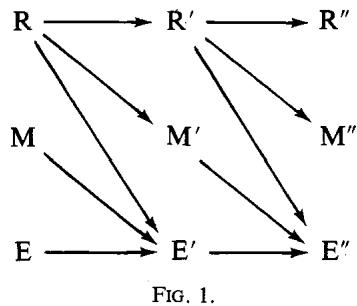
\includegraphics[keepaspectratio]{images/part001_66540ed3.jpg}}

通过上述同构，将H(Homgr \(_A\) (C, C'))等同于Ext (M, M')，同样地，将H(Homgr \(_A\) (C', C''))和H(Homgr \(_A\) (C, C''))也作相应等同，便得到七个同态。

\[
\operatorname{Ext} _ {\mathbf {A}} \left(\mathrm{M} ^ {\prime}, \mathrm{M} ^ {\prime \prime}\right) \otimes_ {k} \operatorname{Ext} _ {\mathbf {A}} \left(\mathrm{M}, \mathrm{M} ^ {\prime}\right)\rightarrow \operatorname{Ext} _ {\mathbf {A}} \left(\mathrm{M}, \mathrm{M} ^ {\prime \prime}\right).
\]

这七个同态彼此一致，并且与分解的选取无关。特别地，它们与第 2 号中通过三元组 (I(M), I(M'), I(M')) 所定义的同态一致。这确实可由将模 H(Homgr (C, C')) 解释为从复形 C 到 C' 的复形态射的同伦类所组成的模，以及以下事实得出：若在复形的一个图中

\[
\begin{array}{c} \mathrm{C} \xrightarrow {f} \mathrm{C} ^ {\prime} \xrightarrow {g} \mathrm{C} ^ {\prime \prime} \\ \alpha \Big \downarrow \qquad \qquad \alpha^ {\prime} \Big \downarrow \qquad \qquad \alpha^ {\prime \prime} \Big \downarrow \\ \mathrm{C} _ {1} \xrightarrow {f _ {1}} \mathrm{C} _ {1} ^ {\prime} \xrightarrow {g _ {1}} \mathrm{C} _ {1} ^ {\prime \prime} \end{array}
\]

\(\alpha'' \circ g\) 同伦于 \(g_1 \circ \alpha'\) ，而 \(\alpha' \circ f\) 同伦于 \(f_1 \circ \alpha\) ，则 \(\alpha'' \circ g \circ f\) 同伦于 \(g_1 \circ f_1 \circ \alpha\) （X，第 33 页，命题 4 及其推论）。

在下文中，我们将视情况使用上述七种复合同态构造中的某一种。

\subsection{与正合列相伴的类}

命题 1. --- 设 (C, d) 和 (C', d') 为两个左 A-模复形，n、p、q 为三个整数，使得 \(p \geqslant q\) 。对于 \(p \geqslant i \geqslant q - 1\) ，设 \(f_i: C_i \to C_{i+n+1}'\) 为一个 A-模同态，使得 \(f_p \circ d = 0\) ， \(f_i \circ d = d' \circ f_{i+1}\) （当 \(p > i \geqslant q - 1\) ），且 \(d' \circ f_{q-1} = 0\) （见图 2）。

\pandocbounded{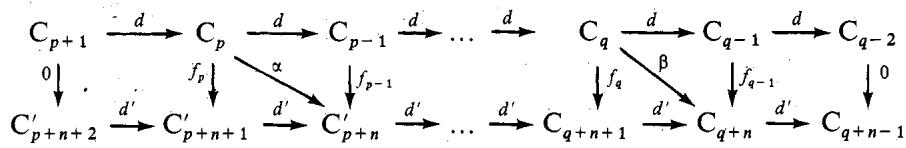
\includegraphics[keepaspectratio]{images/part001_b19b44e0.jpg}}\\
图 2。

令 \(\alpha = f_{p-1} \circ d = d' \circ f_p\) , \(\beta = f_{q-1} \circ d = d' \circ f_q\) ，并设 \(a\) (相应地， \(b\) )为从 C 到 C' 的度为 \(n\) 的分次 A-同态，其仅有的非零双齐次分量是 \(\alpha\) (相应地， \(\beta\) )。则有 \(a \in Z_n(\text{Homgr}_A(C, C'))\) , \(b \in Z_n(\text{Homgr}_A(C, C'))\) 和 \(a - (-1)^{(n+1)(p-q)} b \in B_n(\text{Homgr}_A(C, C'))\) 。

我们有 \(d' \circ \alpha = d' \circ d' \circ f_p = 0\) , \(\alpha \circ d = f_{p-1} \circ d \circ d = 0\) ，因此

\[
a \in Z _ {n} \left(\operatorname{Homgr} _ {\mathrm{A}} \left(\mathrm{C}, \mathrm{C} ^ {\prime}\right)\right);
\]

同理 \(b \in Z_n(\text{Homgr}_A(C, C'))\) 。令 \(\varepsilon = (-1)^{n+1}\) 。在复形 \(\text{Homgr}_A(C, C')\) 中有以下关系

\[
\mathrm{D} f _ {p - 1} = d ^ {\prime} \circ f _ {p - 1} - \varepsilon f _ {p - 1} \circ d = f _ {p - 2} \circ d - \varepsilon \alpha
\]

\[
\mathrm{D} f _ {i} = d ^ {\prime} \circ f _ {i} - \varepsilon f _ {i} \circ d = f _ {i - 1} \circ d - \varepsilon f _ {i} \circ d (p - 1 > i > q)
\]

\[
\mathrm{D} f _ {q} = d ^ {\prime} \circ f _ {q} - \varepsilon f _ {q} \circ d = \beta - \varepsilon f _ {q} \circ d,
\]

因此

\[
\sum_ {i = 1} ^ {p - q} \varepsilon^ {i} D f _ {p - i} = \varepsilon^ {p - q} \beta - \alpha ,
\]

这便证明了引理。

考虑两个左 A-模 M 与 N，以及一个 A-模正合列

\[
0 \rightarrow \mathrm{N} \rightarrow \mathrm{R} _ {n} \rightarrow \mathrm{R} _ {n - 1} \rightarrow \dots \rightarrow \mathrm{R} _ {1} \rightarrow \mathrm{M} \rightarrow 0.\tag{4}
\]

根据 X 第 49 页的命题 3 与命题 3 bis，存在一个交换图：

\begin{enumerate}
\def\labelenumi{(\arabic{enumi})}
\setcounter{enumi}{4}
\tightlist
\item
\end{enumerate}

\pandocbounded{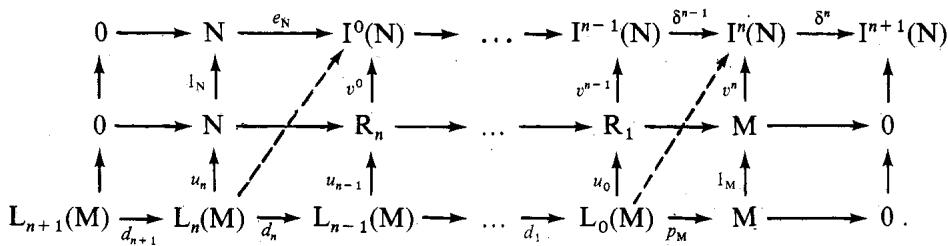
\includegraphics[keepaspectratio]{images/part001_efe78803.jpg}}

考虑这两个元素 \(b\) 与 \(a\) （它们属于 \(\mathrm{Homgr}_{\mathbf{A}}(\mathrm{L}(\mathbf{M}),\mathrm{I}(\mathbf{N}))\) ），其仅有的非零双齐次分量分别是

\[
b ^ {n} = e _ {\mathrm{N}} \circ u _ {n}: \mathrm{L} _ {n} (\mathrm{M}) \rightarrow \mathrm{I} ^ {0} (\mathrm{N}) \quad \text { and } \quad a ^ {n} = v ^ {n} \circ p _ {\mathrm{M}}: \mathrm{L} _ {0} (\mathrm{M}) \rightarrow \mathrm{I} ^ {n} (\mathrm{N})
\]

分别。

命题 2. --- 有 \(a\) , \(b \in Z^n(\text{Homgr}_A (\text{L(M)}, \text{l(N)})\) ）。此外，类 \(\overline{a}\) 与 \(\overline{b}\) ——即 \(a\) 与 \(b\) 的类——在 \(\text{H}^n(\text{Homgr}_A (\text{L(M)}, \text{l(N)})) = \text{Ext}_A^n (\text{M}, \text{N})\) 中仅依赖于正合列 (4)，并且相等。

将命题 1 应用于 (5) 中两端的行以及复合的竖直箭头，取 \(p = n\) , \(q = 0\) ，则有 \(a\) , \(b \in \mathbf{Z}^{n}(\mathrm{Homgr}_{\mathrm{A}}(\mathrm{l(M)}, \mathrm{L(N)}))\) ，并且

\[
a - b = a - (- 1) ^ {(n + 1) n} b \in \mathrm{B} ^ {n} (\operatorname{Homgr} _ {\mathrm{A}} (\mathrm{L} (\mathrm{M}), \mathrm{I} (\mathrm{N}))).
\]

由于 \(a\) （相应地， \(b\) ）与 \(u\) （相应地， \(v\) ）的选取无关，元素 \(\overline{a} = \overline{b}\) （属于 \(\mathrm{Ext}_{\mathbf{A}}^{n}\) (M, N)）与态射 \(u\) 和 \(v\) 的选取无关，由此得出该命题。

定义 1. --- 元素 \(\theta\) ，即 \(\operatorname{Ext}_{\mathbf{A}}^{n}(\mathbf{M}, \mathbf{N})\) 中由 \(\theta = (-1)^{n(n+1)/2} \overline{a} = (-1)^{n(n+1)/2} \overline{b}\) 所定义的元素，称为与正合列 (4) 相伴的类。

注记. --- 1) 设 (P, p) 是 M 的一个投射分解。由 X 第 49 页命题 3，存在一个交换图

\[
\begin{array}{c} 0 \longrightarrow \mathrm{N} \longrightarrow \mathrm{R} _ {n} \longrightarrow \dots \longrightarrow \mathrm{R} _ {1} \longrightarrow \mathrm{M} \longrightarrow 0 \\ \tilde {u} _ {n} \uparrow \quad \tilde {u} _ {n - 1} \uparrow \quad \tilde {u} _ {0} \uparrow \quad \uparrow_ {\mathrm{M}} \\ \mathrm{P} _ {n} \longrightarrow \mathrm{P} _ {n - 1} \longrightarrow \dots \longrightarrow \mathrm{P} _ {0} \xrightarrow {p} \mathrm{M} \longrightarrow 0. \end{array}
\]

使用 § 6 的记号，θ 是态射 P → N 的同伦类在 φ(P, N) 下的像，该态射由 \((-1)^{n(n+1)/2} \tilde{u}_{n}\) 定义。类似地，若 \((e, E)\) 是 N 的一个内射分解，则存在一个交换图

\[
\begin{array}{c} 0 \longrightarrow \mathrm{N} \longrightarrow \mathrm{E} ^ {0} \longrightarrow \dots \longrightarrow \mathrm{E} ^ {n - 1} \longrightarrow \mathrm{E} ^ {n} \\ 1 _ {\mathrm{N}} \uparrow \quad \tilde {v} ^ {0} \uparrow \quad \quad \quad \quad \quad \quad \quad \quad \quad \quad \quad \quad \quad \quad \quad \quad \quad \quad \quad \quad \quad \quad \quad \quad 0 \longrightarrow \mathrm{N} \longrightarrow \mathrm{R} _ {n} \longrightarrow \dots \longrightarrow \mathrm{R} _ {1} \longrightarrow \mathrm{M} \longrightarrow 0. \end{array}
\]

而 \(\theta\) 是 \(\varphi(\mathbf{M},\mathbf{E})\) 下态射 \(\mathbf{M}\to\mathbf{E}\) （由 \((-1)^{n(n+1)/2}v^{n}\) 定义）的同伦类的像。这由 \(\theta\) 的构造以及 \(\varphi(\mathbf{P},\mathbf{N})\) 与 \(\varphi(\mathbf{M},\mathbf{E})\) 的定义得出。

\begin{enumerate}
\def\labelenumi{\arabic{enumi})}
\setcounter{enumi}{1}
\tightlist
\item
  当 \(n = 0\) 时，正合列 (4) 写作 \(0 \to \mathbf{N} \xrightarrow{f} \mathbf{M} \to 0\) ，其相伴类为 \(f^{-1} \in \operatorname{Hom}_{\mathbf{A}}(\mathbf{M}, \mathbf{N}) = \operatorname{Ext}_{\mathbf{A}}^{0}(\mathbf{M}, \mathbf{N})\) 。
\end{enumerate}

\subsection{与正合列相伴的类的性质}

命题 3. --- 设

\begin{enumerate}
\def\labelenumi{(\arabic{enumi})}
\setcounter{enumi}{5}
\tightlist
\item
\end{enumerate}

\[
0 \rightarrow \mathrm{P} \rightarrow \mathrm{S} _ {m} \rightarrow \mathrm{S} _ {m - 1} \rightarrow \dots \rightarrow \mathrm{S} _ {1} \stackrel {\lambda_ {n}} {\rightarrow} \mathrm{N} \rightarrow 0\tag{7}
\]

\[
0 \rightarrow \mathrm{N} \xrightarrow {\mu} \mathrm{R} _ {n} \rightarrow \mathrm{R} _ {n - 1} \rightarrow \dots \rightarrow \mathrm{R} _ {1} \rightarrow \mathrm{M} \rightarrow 0
\]

为两个左 A-模正合列，其类分别为 \(\theta\in\mathrm{Ext}_{\mathbf{A}}^{m}(\mathbf{N},\mathbf{P})\) 与 \(\theta^{\prime}\in\mathrm{Ext}_{\mathbf{A}}^{n}(\mathbf{M},\mathbf{N})\) 。 \(\mathrm{Ext}_{\mathbf{A}}^{m+n}(\mathbf{M},\mathbf{P})\) 中与正合列

\[
0 \to \mathrm{P} \to \mathrm{S} _ {m} \to \dots \to \mathrm{S} _ {1} \xrightarrow {\mu \circ \lambda} \mathrm{R} _ {n} \to \dots \to \mathrm{R} _ {1} \to \mathrm{M} \to 0\tag{8}
\]

相伴的类是复合积 \(\theta\circ\theta'\) 。

选取交换图

\[
\begin{array}{c} 0 \longrightarrow \mathrm{P} \longrightarrow \mathrm{I} ^ {0} (\mathrm{P}) \longrightarrow \dots \longrightarrow \mathrm{I} ^ {m - 1} (\mathrm{P}) \xrightarrow {\delta_ {\mathrm{P}} ^ {m - 1}} \mathrm{I} ^ {m} (\mathrm{P}) \\ 0 \longrightarrow \mathrm{P} \longrightarrow \mathrm{S} _ {m} \longrightarrow \dots \longrightarrow \mathrm{S} _ {1} \xrightarrow {\lambda} \mathrm{N} \longrightarrow 0, \end{array}
\]

\[
\begin{array}{c c c c c c c c c c c c} 0 \longrightarrow & \mathrm{N} & \stackrel {{e _ {\mathrm{N}}}} {{\longrightarrow}} & \mathrm{I} ^ {0} (\mathrm{N}) & \longrightarrow & \dots & \longrightarrow & \mathrm{I} ^ {n - 1} (\mathrm{N}) & \longrightarrow & \mathrm{I} ^ {n} (\mathrm{N}) \\ & \uparrow_ {1 _ {\mathrm{N}}} & & v ^ {0} \uparrow & & & & v ^ {n - 1} \uparrow & & v ^ {n} \uparrow \\ 0 \longrightarrow & \mathrm{N} & \stackrel {{\mu}} {{\longrightarrow}} & \mathrm{R} _ {n} & \longrightarrow & \dots & \longrightarrow & \mathrm{R} _ {1} & \longrightarrow & \mathrm{M} & \longrightarrow & 0. \end{array}
\]

由于 \(\mathrm{I}^{m}(\mathrm{P})\) 是内射的，存在同态 \(h^{0}: \mathrm{I}^{0}(\mathrm{N}) \to \mathrm{I}^{m}(\mathrm{P})\) 使得 \(w^{m} = h^{0} \circ e_{N}\) ；由 X 第 49 页命题 3 bis， \(h^{0}\) 可延拓为复形的态射 \(h: \mathrm{I}(\mathrm{N}) \to \mathrm{I}(\mathrm{P})(-m)\) 。于是 \(w^{m} = h^{0} \circ e_{N} = h^{0} \circ v^{0} \circ \mu\) ，因此

\[
\delta_ {1} ^ {m - 1} \circ w ^ {m - 1} = w ^ {m} \circ \lambda = h ^ {0} \circ v ^ {0} \circ (\mu \circ \lambda),
\]

且下图是交换的：

\[
\begin{array}{l}0 \longrightarrow \mathrm{P} \longrightarrow \mathrm{I} ^ {0} (\mathrm{P}) \longrightarrow \dots \longrightarrow \mathrm{I} ^ {m - 1} (\mathrm{P}) \longrightarrow \mathrm{I} ^ {m} (\mathrm{P}) \longrightarrow \mathrm{I} ^ {m + 1} (\mathrm{P}) \longrightarrow \dots \longrightarrow \mathrm{I} ^ {m + n} (\mathrm{P})\\0 \longrightarrow \mathrm{P} \longrightarrow \mathrm{S} _ {m} \longrightarrow \dots \longrightarrow \mathrm{S} _ {1} \underset {\mu \circ \lambda} {\longrightarrow} \mathrm{R} _ {n} \longrightarrow \mathrm{R} _ {n - 1} \longrightarrow \dots \longrightarrow \mathrm{M} \rightarrow 0\end{array}
\]

其中 \(t^0 = h^0 \circ v^0\) , \(t^1 = (-1)^m h^1 \circ v^1, \ldots, t^i = (-1)^{mi} h^i \circ v^i, \ldots, t^n = (-1)^{mn} h^n \circ v^n\) 。与 (6) 相伴的类 \(\theta\) 是 \((-1)^{m(m+1)/2} w^m \in \text{Homgr}_A^m(\mathbf{N}, \mathbf{l}(\mathbf{P}))\) 的类，因此经同构 \(a_{\mathbf{N},\mathbf{P}}\) 对应于 \((-1)^{m(m+1)/2} h \in \text{Homgr}_A^m(\mathbf{l}(\mathbf{N}), \mathbf{l}(\mathbf{P}))\) 的类；与 (7) 相伴的类 \(\theta'\) 是 \((-1)^{n(n+1)/2} v^n \in \text{Homgr}_A^m(\mathbf{M}, \mathbf{l}(\mathbf{N}))\) 的类，与 (8) 相伴的类是 \((-1)^{(m+n)(m+n+1)/2} t^n \in \text{Homgr}_{m+n}^m(\mathbf{M}, \mathbf{l}(\mathbf{P}))\) 的类，于是由复合积的定义（X，第 114 页）及公式得出结论

\[
m (m + 1) / 2 + n (n + 1) / 2 = (m + n) (m + n + 1) / 2 - m n.
\]

\begin{enumerate}
\def\labelenumi{\arabic{enumi}.}
\setcounter{enumi}{3}
\tightlist
\item
  --- 考虑一个 A-模的交换图，它具有正合
\end{enumerate}

行

\pandocbounded{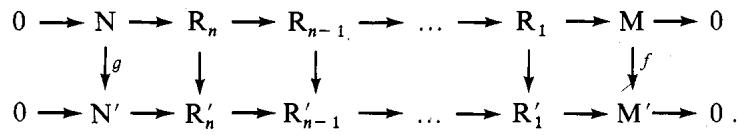
\includegraphics[keepaspectratio]{images/part001_b790ce53.jpg}}

设 θ（相应地，θ′）为第一行（相应地，第二行）在下式中的类

\[
\operatorname{Ext} _ {\mathbf {A}} ^ {n} (\mathbf {M}, \mathbf {N}) \quad \left(\text { resp.   } \operatorname{Ext} _ {\mathbf {A}} ^ {n} (\mathbf {M} ^ {\prime}, \mathbf {N} ^ {\prime})\right).
\]

在 \(\operatorname{Ext}_{\mathbf{A}}^{n}(\mathbf{M}, \mathbf{N}')\) 中，有 \(\theta' \circ f = g \circ \theta\) 。

事实上，考虑一个交换图

\pandocbounded{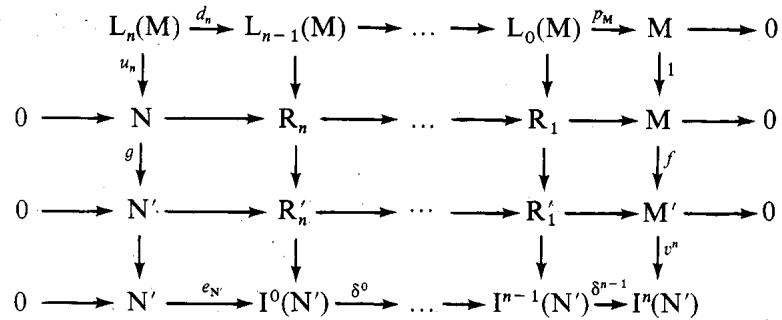
\includegraphics[keepaspectratio]{images/part001_126cf8d3.jpg}}

根据定义， \(\theta' \circ f\) 是 \((-1)^{n(n+1)/2} v^n \circ f \circ p_M \in \text{Homgr}^n (\text{L(M)}, \text{I(N')})\) 的类，而 \(g \circ \theta\) 是 \((-1)^{n(n+1)/2} e_{N'} \circ g \circ u_n\) 的类。将引理 1 应用于该图两端的行，这两个类相等。

推论 1. --- 考虑一个具有正合行的交换图

\[
\begin{array}{c c c c c c c c} 0 \longrightarrow & \mathrm{N} \longrightarrow & \mathrm{R} _ {n} \longrightarrow & \dots & \longrightarrow & \mathrm{R} _ {1} \longrightarrow & \mathrm{M} \longrightarrow & 0 \\ & ^ {1} \downarrow & & & \downarrow & & ^ {1} \downarrow \\ 0 \longrightarrow & \mathrm{N} \longrightarrow & \mathrm{R} _ {n} ^ {\prime} \longrightarrow & \dots & \longrightarrow & \mathrm{R} _ {1} ^ {\prime} \longrightarrow & \mathrm{M} \longrightarrow & 0; \end{array}
\]

图的两行在 \(\operatorname{Ext}_{\mathbf{A}}^{n}(\mathbf{M},\mathbf{N})\) 中有相同的相伴类。

推论 2. --- 设

\[
0 \rightarrow \mathrm{N} \xrightarrow {f _ {n - 1}} \mathrm{R} _ {n} \xrightarrow {f _ {n}} \mathrm{R} _ {n - 1} \rightarrow \dots \xrightarrow {f _ {2}} \mathrm{R} _ {1} \xrightarrow {f _ {1}} \mathrm{M} \rightarrow 0
\]

是一个正合列， \(\theta\in\mathrm{Ext}_{\mathbf{A}}^{n}(\mathbf{M},\mathbf{N})\) 为其相伴的类， \(a_{1},\ldots,a_{n+1}\) 为 \(k\) 的可逆元。与正合列

\[
0 \rightarrow \mathrm{N} \xrightarrow {a _ {n + 1} f _ {n + 1}} \mathrm{R} _ {n} \xrightarrow {a _ {n} f _ {n}} \mathrm{R} _ {n - 1} \rightarrow \dots \xrightarrow {a _ {2} f _ {2}} \mathrm{R} _ {1} \xrightarrow {a _ {1} f _ {1}} \mathrm{M} \rightarrow 0
\]

相伴的类是 \((a_{1}^{-1}a_{2}^{-1}\dots a_{n + 1}^{-1})\theta .\)

事实上，我们有一个交换图

\[
\begin{array}{c} 0 \longrightarrow \mathrm{N} \xrightarrow {a _ {n + 1} f _ {n + 1}} \mathrm{R} _ {n} \longrightarrow \dots \longrightarrow \mathrm{R} _ {2} \xrightarrow {a _ {2} f _ {2}} \mathrm{R} _ {1} \xrightarrow {a _ {1} f _ {1}} \mathrm{M} \longrightarrow 0 \\ \Biggl \downarrow a _ {1} \dots a _ {n + 1} \quad \Biggl \downarrow a _ {1} \dots a _ {n} \quad \Biggl \downarrow a _ {1} a _ {2} \quad \Biggl \downarrow a _ {1} \quad \Biggl \downarrow 1 \\ 0 \longrightarrow \mathrm{N} \xrightarrow {f _ {n + 1}} \mathrm{R} _ {n} \longrightarrow \dots \longrightarrow \mathrm{R} _ {2} \xrightarrow {f _ {2}} \mathrm{R} _ {1} \xrightarrow {f _ {1}} \mathrm{M} \longrightarrow 0. \end{array}
\]

然后应用该命题。

推论 3. --- 设 \(0 \to \mathbf{N} \xrightarrow{f_{n+1}} \mathbf{R}_{n} \xrightarrow{f_{n}} \cdots \to \mathbf{R}_{1} \xrightarrow{f_{1}} \mathbf{M} \to 0\) 为一个正合列， \(\theta\) 为它在 \(\operatorname{Ext}_{\mathbf{A}}^{n}(\mathbf{M}, \mathbf{N})\) 中的类， \(u: \mathbf{M}' \to \mathbf{M}\) 与 \(v: \mathbf{N} \to \mathbf{N}'\) 为两个 A-模同态。

\begin{enumerate}
\def\labelenumi{\alph{enumi})}
\tightlist
\item
  元素 \(v \circ \theta\) （属于 \(\operatorname{Ext}_{\mathbf{A}}^{n}(\mathbf{M}, \mathbf{N}')\) ）等于正合列
\end{enumerate}

\[
0 \rightarrow \mathrm{N} ^ {\prime} \xrightarrow {f _ {n + 1} ^ {\prime}} \mathrm{R} _ {n} ^ {\prime} \xrightarrow {f _ {n} ^ {\prime}} \mathrm{R} _ {n - 1} \xrightarrow {f _ {n - 1}} \dots \rightarrow \mathrm{R} _ {1} \rightarrow \mathrm{M} \rightarrow 0,
\]

的类，其中 \(R_{n}^{\prime}\) 是 A-模 \(R_{n} \oplus N^{\prime}\) 除以由诸对 \((f_{n+1}(x), -v(x))\) （ \(x \in N\) ）所构成的子模而得的商模，而 \(f_{n+1}^{\prime}\) (相应地， \(f_{n}^{\prime}\) )由典范单射（相应地，由 \((f_{n}, 0)\) ）通过取商得到。

\begin{enumerate}
\def\labelenumi{\alph{enumi})}
\setcounter{enumi}{1}
\tightlist
\item
  元素 \(\theta \circ u\) （属于 \(\operatorname{Ext}_{\mathbf{A}}^{n}(\mathbf{M}^{\prime}, \mathbf{N})\) ）是正合列
\end{enumerate}

\[
0 \rightarrow \mathrm{N} \rightarrow \mathrm{R} _ {n} \rightarrow \dots \rightarrow \mathrm{R} _ {2} \xrightarrow {f _ {2} ^ {\prime \prime}} \mathrm{R} _ {1} ^ {\prime} \xrightarrow {f _ {1} ^ {\prime \prime}} \mathrm{M} ^ {\prime} \rightarrow 0,
\]

的类，其中 \(R_{1}^{\prime}\) 是纤维积 \(R_{1} \times_{M} M^{\prime}\) ，亦即（I，第 44 页） \(R_{1} \times M^{\prime}\) 中由对 \((x, y)\) （满足 \(f_{1}(x) = u(y)\) ）所构成的子模，而 \(f_{2}^{\prime\prime}\) (相应地， \(f_{1}^{\prime\prime}\) )由 \((f_{2}, 0)\) （相应地，由第二个投影）导出。

例如，我们来证明 \(a\) )。设 \(z\) 为 \(\mathbf{R}_{n}^{\prime}\) 中满足 \(f_{n}^{\prime}(z)=0\) 的一个元素；若 \(z\) 是对 \((x,y)\) 的类，其中 \(x\in\mathbf{R}_{n},y\in\mathbf{N}^{\prime}\) ，则有 \(f_{n}(x)=0\) ，从而存在元素 \(t\in\mathbf{N}\) 使得 \(x=f_{n+1}(t)\) 。于是有 \(z=f_{n+1}^{\prime}(y+v(t))\) ，这就证明了 \(\operatorname{Ker} f_{n}^{\prime}=\operatorname{Im} f_{n+1}^{\prime}\) 。 \(f_{n+1}^{\prime}\) 的单射性由 \(f_{n+1}\) 的单射性得出。

设 \(j: \mathbf{R}_{n} \to \mathbf{R}_{n}^{\prime}\) 为由典范单射导出的同态；我们有正合列的交换图：

\[
\begin{array}{c} 0 \longrightarrow \mathrm{N} \xrightarrow {f _ {n + 1}} \mathrm{R} _ {n} \xrightarrow {f _ {n}} \mathrm{R} _ {n - 1} \longrightarrow \dots \longrightarrow \mathrm{M} \longrightarrow 0 \\ \Biggl \downarrow v \quad \Biggl \downarrow j \quad \Biggl \downarrow 1 \\ 0 \longrightarrow \mathrm{N} ^ {\prime} \xrightarrow {f _ {n + 1} ^ {\prime}} \mathrm{R} _ {n} ^ {\prime} \xrightarrow {f _ {n} ^ {\prime}} \mathrm{R} _ {n - 1} \longrightarrow \dots \longrightarrow \mathrm{M} \longrightarrow 0; \end{array}
\]

于是断言 a) 由该命题得出。

 \(b\) 的证明是类似的。

注记。--- 设 \(\theta\in\mathrm{Ext}_{\mathbf{A}}^{n}(\mathbf{M},\mathbf{N})\) ，分别地 \(\theta^{\prime}\in\mathrm{Ext}_{\mathbf{A}}^{n}(\mathbf{M}^{\prime},\mathbf{N}^{\prime})\) ，是正合序列的类

\[
0 \rightarrow \mathrm{N} \xrightarrow {f _ {n + 1}} \mathrm{R} _ {n} \rightarrow \dots \rightarrow \mathrm{R} _ {1} \xrightarrow {f _ {1}} \mathrm{M} \rightarrow 0,
\]

\[
\text { resp. } 0 \to \mathrm{N} ^ {\prime} \xrightarrow {f _ {n + 1} ^ {\prime}} \mathrm{R} _ {n} ^ {\prime} \to \dots \to \mathrm{R} _ {1} ^ {\prime} \xrightarrow {f _ {1} ^ {\prime}} \mathrm{M} ^ {\prime} \to 0.
\]

设 \(i_{\mathbf{N}}, i_{\mathbf{N}'}\) 为 \(\mathbf{N}\) 与 \(\mathbf{N}'\) 到 \(\mathbf{N} \oplus \mathbf{N}'\) 中的典范单射， \(q_{\mathbf{M}}\) , \(q_{\mathbf{M}'}\) 为 \(\mathbf{M} \oplus \mathbf{M}'\) 到 \(\mathbf{M}\) 与 \(\mathbf{M}'\) 上的投影。考虑同态

\[
m = \operatorname{Ext} \left(q _ {\mathbf {M}}, i _ {\mathbf {N}}\right) \oplus \operatorname{Ext} \left(q _ {\mathbf {M} ^ {\prime}}, i _ {\mathbf {N} ^ {\prime}}\right)
\]

是从 \(\operatorname{Ext}_{\mathbf{A}}(\mathbf{M},\mathbf{N})\oplus \operatorname{Ext}_{\mathbf{A}}(\mathbf{M}^{\prime},\mathbf{N}^{\prime})\) 到 \(\operatorname{Ext}_{\mathbf{A}}(\mathbf{M}\oplus \mathbf{M}^{\prime},\mathbf{N}\oplus \mathbf{N}^{\prime}\) 的同态。元素

\[
m (\theta , \theta^ {\prime}) = i _ {\mathrm{N}} \circ \theta \circ q _ {\mathrm{M}} + i _ {\mathrm {N^ {\prime}}} \circ \theta^ {\prime} \circ q _ {\mathrm {M^ {\prime}}}
\]

是正合列

\[
0 \rightarrow \mathrm{N} \oplus \mathrm{N} ^ {\prime} \xrightarrow {f _ {n + 1} \oplus f _ {n - 1} ^ {\prime}} \mathrm{R} _ {n} \oplus \mathrm{R} _ {n} ^ {\prime} \rightarrow \dots \rightarrow \mathrm{R} _ {1} \oplus \mathrm{R} _ {1} ^ {\prime} \xrightarrow {f _ {1} \oplus f _ {1} ^ {\prime}} \mathrm{M} \oplus \mathrm{M} ^ {\prime} \rightarrow 0.
\]

的类。事实上，若将这个类记为 \(\theta''\) ，则由命题 4 可知，有

\[
\theta^ {\prime \prime} \circ i _ {\mathrm{M}} = i _ {\mathrm{N}} \circ \theta = m (\theta , \theta^ {\prime}) \circ i _ {\mathrm{M}} \quad \text {and} \quad \theta^ {\prime \prime} \circ i _ {\mathrm{M} ^ {\prime}} = i _ {\mathrm{N} ^ {\prime}} \circ \theta = m (\theta , \theta^ {\prime}) \circ i _ {\mathrm{M} ^ {\prime}};
\]

根据 X 第 89 页命题 7，这意味着 \(\theta'' = m(\theta, \theta')\) 。

\subsection{\texorpdfstring{正合列与 Ext 元素之间的关系 \(_{A}\) (M, N)}{正合列与 Ext 元素之间的关系 \_\{A\} (M, N)}}

定理 1. --- 设 n 为整数 ≥1，M 和 N 为两个 A-模。

\begin{enumerate}
\def\labelenumi{\alph{enumi})}
\item
  Ext \(_{A}^{n}\) (M, N) 的每个元素都是某个正合列的类（X，第 117 页，定义 1）。
\item
  设 \(0 \to \mathbf{N} \xrightarrow{f_{n+1}} \mathbf{R}_n \xrightarrow{f_n} \ldots \to \mathbf{R}_1 \xrightarrow{f_1} \mathbf{M} \to 0\)
\end{enumerate}

和

\[
0 \rightarrow \mathrm{N} \xrightarrow {f _ {n + 1} ^ {\prime}} \mathrm{R} _ {n} ^ {\prime} \xrightarrow {f _ {n} ^ {\prime}} \dots \rightarrow \mathrm{R} _ {1} ^ {\prime} \xrightarrow {f _ {1} ^ {\prime}} \mathrm{M} \rightarrow 0
\]

为两个正合列， \(\theta\) 与 \(\theta'\) 为其相伴的类。以下条件等价：

\begin{enumerate}
\def\labelenumi{(\roman{enumi})}
\item
  \(\theta = \theta^{\prime}\) ;
\item
  存在一个具有正合行的交换图：
\end{enumerate}

\[
\begin{array}{c} 0 \longrightarrow \mathrm{N} \xrightarrow {f _ {n + 1}} \mathrm{R} _ {n} \longrightarrow \dots \longrightarrow \mathrm{R} _ {1} \xrightarrow {f _ {1}} \mathrm{M} \longrightarrow 0 \\ 0 \longrightarrow \mathrm{N} \longrightarrow \mathrm{R} _ {n} ^ {\prime \prime} \longrightarrow \dots \longrightarrow \mathrm{R} _ {1} ^ {\prime} \longrightarrow \mathrm{M} \longrightarrow 0 \\ 0 \longrightarrow \mathrm{N} \xrightarrow {f _ {n + 1} ^ {\prime}} \mathrm{R} _ {n} ^ {\prime} \longrightarrow \dots \longrightarrow \mathrm{R} _ {1} ^ {\prime} \xrightarrow {f _ {1} ^ {\prime}} \mathrm{M} \longrightarrow 0; \end{array}
\]

\begin{enumerate}
\def\labelenumi{(\roman{enumi})}
\setcounter{enumi}{2}
\tightlist
\item
  存在一个具有正合行的交换图：
\end{enumerate}

\[
\begin{array}{c} 0 \longrightarrow \mathrm{N} \xrightarrow {f _ {n + 1}} \mathrm{R} _ {n} \longrightarrow \dots \longrightarrow \mathrm{R} _ {1} \xrightarrow {f _ {1}} \mathrm{M} \longrightarrow 0 \\ 0 \longrightarrow \mathrm{N} \longrightarrow \mathrm{R} _ {n} ^ {\prime \prime} \longrightarrow \dots \longrightarrow \mathrm{R} _ {1} ^ {\prime \prime} \longrightarrow \mathrm{M} \longrightarrow 0 \\ 0 \longrightarrow \mathrm{N} \xrightarrow {f _ {n + 1} ^ {\prime}} \mathrm{R} _ {n} ^ {\prime} \longrightarrow \dots \longrightarrow \mathrm{R} _ {1} ^ {\prime} \xrightarrow {f _ {1} ^ {\prime}} \mathrm{M} \longrightarrow 0. \end{array}
\]

我们来证明 \(a\) )。设 \(\alpha \in \operatorname{Ext}_{\mathbf{A}}^{n}(\mathbf{M}, \mathbf{N})\) ，并设 \(\mathbf{P}\) 为 \(\mathbf{M}\) 的一个投射分解。设 \(a: \mathrm{P}(n) \to \mathbf{N}\) 为表示 \(\alpha\) 的复形态射；其唯一的非零分量是一个 A-同态 \(u: \mathrm{P}_{n} \to \mathbf{N}\) ，它满足 \(u \circ d_{n+1} = 0\) ，因此有分解 \(u = \overline{u} \circ \delta_{n}\) ，其中 \(\delta_{n}: \mathrm{P}_{n} \to \dot{\mathbf{Z}}_{n-1}\) 是由 \(d_{n}\) 诱导的映射（我们设 \(Z_{n-1} = \operatorname{Im} d_{n}\) ），而 \(\overline{u}\) 是从 \(Z_{n-1}\) 到 \(\mathbf{N}\) 的一个 A-同态。根据第 117 页的注记 1，类 \(\theta \in \operatorname{Ext}_{\mathbf{A}}^{n}(\mathbf{M}, Z_{n-1})\) ——即正合列

\[
0 \rightarrow Z _ {n - 1} \rightarrow P _ {n - 1} \rightarrow \dots \rightarrow P _ {0} \rightarrow M \rightarrow 0
\]

的类——等于态射 \((-1)^{n(n + 1) / 2}\delta_n\) 的同伦类。因此我们有

\[
\alpha = (- 1) ^ {n (n + 1) / 2} \overline {{{u}}} \circ \theta ,
\]

根据第 120 页的推论 3，由此可将 α 表示为某个正合列的类。

由 X 第 120 页的推论 1 可知，(ii) \(\Rightarrow\) (i) 且 (iii) \(\Rightarrow\) (i)。假设 (i) 成立，并设 P 为 M 的一个投射分解。存在一个交换图

\[
\begin{array}{c} 0 \longrightarrow \mathrm{N} \xrightarrow {f _ {n + 1}} \mathrm{R} _ {n} \longrightarrow \mathrm{R} _ {n - 1} \longrightarrow \dots \longrightarrow \mathrm{R} _ {1} \longrightarrow \mathrm{M} \longrightarrow 0 \\ u _ {n} \uparrow \quad \uparrow u _ {n - 1} \quad \uparrow u _ {n - 2} \quad \uparrow \quad \uparrow_ {\mathrm{I} _ {\mathrm{M}}} \\ \mathrm{P} _ {n} \xrightarrow {d _ {n}} \mathrm{P} _ {n - 1} \longrightarrow \mathrm{P} _ {n - 2} \longrightarrow \dots \longrightarrow \mathrm{P} _ {0} \longrightarrow \mathrm{M} \longrightarrow 0 \\ u _ {n} ^ {\prime} \downarrow \quad \downarrow u _ {n - 1} ^ {\prime} \quad \downarrow u _ {n - 2} ^ {\prime} \quad \downarrow \quad \downarrow_ {\mathrm{I} _ {\mathrm{M}}} \\ 0 \longrightarrow \mathrm{N} \xrightarrow {f _ {n + 1}} \mathrm{R} _ {n} ^ {\prime} \longrightarrow \mathrm{R} _ {n - 1} ^ {\prime} \longrightarrow \dots \longrightarrow \mathrm{R} _ {1} ^ {\prime} \longrightarrow \mathrm{M} \longrightarrow 0. \end{array}
\]

从 \(\mathrm{P}(n)\) 到 \(\mathbf{N}\) 的、由 \(u_{n}\) 与 \(u_{n}^{\prime}\) 定义的态射是同伦的，因为它们都属于类 \((-1)^{n(n + 1) / 2}\theta\) ，因此 \(u_{n}^{\prime} - u_{n}\) 具有 \(w\circ d_n\) 的形式，其中 \(w:\mathrm{P}_{n - 1}\to \mathrm{N}\) 是一个 A-同态。将 \(u_{n - 1}^{\prime}\) 换为 \(u_{n - 1}^{\prime} - f_{n + 1}^{\prime}\circ w\) ，并将 \(u_{n}^{\prime}\) 换为 \(u_{n}\) ，就可归结为 \(u_{n} = u_{n}^{\prime}\) 的情形。这使得我们可以构造一个新的具有正合行的交换图：

\[
\begin{array}{c c c c c c c} 0 \longrightarrow \mathrm{N} \longrightarrow \mathrm{R} _ {n} \longrightarrow \mathrm{R} _ {n - 1} \longrightarrow \dots \longrightarrow \mathrm{R} _ {1} \longrightarrow \mathrm{M} \longrightarrow 0 \\ 1 _ {\mathrm{N}} \uparrow & \uparrow v & \uparrow u _ {n - 2} & \uparrow & \uparrow^ {1 _ {\mathrm{M}}} \\ 0 \longrightarrow \mathrm{N} \longrightarrow \mathrm{N} ^ {\prime} \longrightarrow \mathrm{P} _ {n - 2}. \longrightarrow \dots \longrightarrow \mathrm{P} _ {0} \longrightarrow \mathrm{M} \longrightarrow 0 \\ 1 _ {\mathrm{N}} \downarrow & \downarrow v ^ {\prime} & \downarrow u _ {n - 2} ^ {\prime} & \downarrow & \downarrow^ {1 _ {\mathrm{M}}} \\ 0 \longrightarrow \mathrm{N} \longrightarrow \mathrm{R} _ {n} ^ {\prime} \longrightarrow \mathrm{R} _ {n - 1} ^ {\prime} \longrightarrow \dots \longrightarrow \mathrm{R} _ {1} ^ {\prime} \longrightarrow \mathrm{M} \longrightarrow 0 \end{array}
\]

其中 \(\mathbf{N}'\) 是 \(\mathbf{P}_{n-1} \oplus \mathbf{N}\) 除以由诸对 \((d_n(x), -u_n(x))\) （ \(x \in \mathbf{P}_n\) ）所构成的子模而得的商模，而 \(v\) (相应地， \(v'\) )是由映射 \(u_{n-1} \oplus f_{n+1}\) （相应地， \(u_{n-1}' \oplus f_{n+1}'\) ）通过取商定义的。因此条件 (ii) 得到满足。

再假设条件 (i) 成立，并设 E 为 N 的一个内射分解。存在一个交换图

\[
\begin{array}{c c c c c c c} 0 \longrightarrow \mathrm{N} \longrightarrow \mathrm{R} _ {n} \longrightarrow & \dots \longrightarrow \mathrm{R} _ {1} \longrightarrow \mathrm{M} \longrightarrow & 0 \\ 1 _ {\mathrm{N}} \Big \downarrow & \Big \downarrow v _ {0} & v _ {n - 1} \Big \downarrow & \Big \downarrow v _ {n} \\ 0 \longrightarrow \mathrm{N} ^ {\prime} \longrightarrow \mathrm{E} ^ {0} \stackrel {{\delta^ {0}}} {{\longrightarrow}} & \dots \longrightarrow \mathrm{E} ^ {n - 1} \stackrel {{\delta^ {n - 1}}} {{\longrightarrow}} \mathrm{E} ^ {n} \\ 1 _ {\mathrm{N}} \Big \uparrow & \Big \uparrow v _ {0} ^ {\prime} & v _ {n - 1} ^ {\prime} \Big \uparrow & \Big \uparrow v _ {n} ^ {\prime} \\ 0 \longrightarrow \mathrm{N} \longrightarrow \mathrm{R} _ {n} ^ {\prime} \longrightarrow & \dots \longrightarrow \mathrm{R} _ {1} ^ {\prime} \longrightarrow & \mathrm{M} \longrightarrow & 0 \end{array}
\]

并且如上面所示，可以假设 \(v_{n}^{\prime}=v_{n}\) 。于是我们有一个具有正合行的交换图

\[
\begin{array}{c c c c c c c c} 0 \longrightarrow N \longrightarrow R _ {n} \longrightarrow \dots \longrightarrow R _ {2} \longrightarrow R _ {1} \longrightarrow M \longrightarrow 0 \\ \downarrow^ {1 _ {N}} & \downarrow & & \downarrow & \downarrow & \downarrow^ {1 _ {M}} \\ 0 \longrightarrow N \longrightarrow E ^ {0} \longrightarrow \dots \longrightarrow E ^ {n - 2} \longrightarrow M ^ {\prime} \longrightarrow M \longrightarrow 0 \\ \uparrow^ {1 _ {N}} & \uparrow & & \uparrow & \uparrow & \uparrow^ {1 _ {M}} \\ 0 \longrightarrow N \longrightarrow R _ {n} ^ {\prime} \longrightarrow \dots \longrightarrow R _ {2} ^ {\prime} \longrightarrow R _ {1} ^ {\prime} \longrightarrow M \longrightarrow 0 \end{array}
\]

其中 \(\mathbf{M}' = \mathbf{M} \times_{\mathrm{R}_{1}} \mathbf{E}_{n-1}\) （参见 X，第 120 页，推论 3，b））。因此条件 (iii) 成立，这就完成了定理的证明。

注记 1. --- 若环 A 是诺特环，且 A-模 M 与 N 都是有限生成的，则由 a) 的证明可知，Ext \(_{A}^{n}\) (M, N) 的每个元素都是与某个正合列 0 → N → R \(_{n}\) → \ldots{} → R \(_{1}\) → M → 0 相伴的类，其中诸 R \(_{i}\) 都是有限生成的。

推论. --- 设 \(0 \to \mathbf{N} \xrightarrow{f} \mathbf{R} \xrightarrow{g} \mathbf{M} \to 0\) 与 \(0 \to \mathbf{N} \xrightarrow{f'} \mathbf{R}' \xrightarrow{g'} \mathbf{M} \to 0\) 为两个正合列， \(\theta\) 与 \(\theta'\) 为它们在 \(\operatorname{Ext}^1(\mathbf{M}, \mathbf{N})\) 中的相伴类。为使 \(\theta = \theta'\) ，必须且只需存在一个 A-同态 \(h: \mathbf{R} \to \mathbf{R}'\) 使得图表

\[
\begin{array}{c} \mathsf {R} \\ \mathsf {N} \\ \mathsf {f ^ {\prime}} \end{array} \begin{array}{c} \mathsf {f} \\ \mathsf {h} \\ \mathsf {R ^ {\prime}} \end{array} \begin{array}{c} \mathsf {g} \\ \mathsf {M} \\ \mathsf {g ^ {\prime}} \end{array}
\]

交换的。这样的同态必然是一个同构。

由命题 4 的推论 1，该条件是充分的。若 \(\theta = \theta'\) ，则我们有一个具有正合行的交换图：

\[
\begin{array}{c} 0 \longrightarrow \mathrm{N} \longrightarrow \mathrm{R} \longrightarrow \mathrm{M} \longrightarrow 0 \\ \uparrow_ {1 _ {\mathrm{N}}} \Big | _ {h ^ {\prime}} \Big | _ {1 _ {\mathrm{M}}} \\ 0 \longrightarrow \mathrm{N} \longrightarrow \mathrm{R} ^ {\prime \prime} \longrightarrow \mathrm{M} \longrightarrow 0 \\ \uparrow_ {1 _ {\mathrm{N}}} \Big | _ {h ^ {\prime \prime}} \Big | _ {1 _ {\mathrm{M}}} \\ 0 \longrightarrow \mathrm{N} \longrightarrow \mathrm{R} ^ {\prime} \longrightarrow \mathrm{M} \longrightarrow 0. \end{array}
\]

态射 \(h'\) 与 \(h''\) 由 X 第 7 页推论 3 知是同构，且 \(h = h'' \circ h'^{-1}\) 回答了该问题。最后一个断言由同上引文得出。

注记 2. --- 定理 1 把 Ext \(_{A}^{n}\) (M, N) 描述为正合列的等价类集合；通过结构转移，容易描述在此集合上得到的群法则。事实上，设 θ（相应地，θ′）为正合列 0 → N \(\xrightarrow{f_{n+1}}\) R \(_{n}\) \(\xrightarrow{f_n}\) \ldots{} → R \(_{1}\) → M → 0（相应地，0 → N \(\xrightarrow{f_{n+1}'}\) R \(_{n}'\) \(\xrightarrow{f_n'}\) \ldots{} → R \(_{1}'\) → M → 0）的类。设 Δ : M → M ⊕ M 与 ∇ : N ⊕ N → N 为 A-线性映射，由 Δ(x) = (x, x)（x ∈ M）与 ∇(y, z) = y + z（y, z ∈ N）定义。考虑映射

\[
m: \operatorname{Ext} _ {\mathbf {A}} (\mathbf {M}, \mathbf {N}) \oplus \operatorname{Ext} _ {\mathbf {A}} (\mathbf {M}, \mathbf {N}) \rightarrow \operatorname{Ext} _ {\mathbf {A}} (\mathbf {M} \oplus \mathbf {M}, \mathbf {N} \oplus \mathbf {N})
\]

是在第 121 页的注记中定义的。采用同上引文的记号，我们有 \(\nabla \circ i_{\mathbf{N}} = 1_{\mathbf{N}}\) 和 \(q_{\mathbf{M}} \circ \Delta = 1_{\mathbf{M}}\) ，从而 \(\theta + \theta' = \nabla \circ m(\theta, \theta') \circ \Delta\) 。鉴于同上引文及第 120 页的推论 3，这就给出一个类为 \(\theta + \theta'\) 的正合列：例如，若 \(n \geqslant 2\) ，可取序列

\[
0 \rightarrow \mathrm{N} \rightarrow \mathrm{R} _ {n} ^ {\prime \prime} \rightarrow \mathrm{R} _ {n - 1} \oplus \mathrm{R} _ {n - 1} ^ {\prime} \xrightarrow {f _ {n - 1} \oplus f _ {n - 1} ^ {\prime}} \dots \rightarrow \mathrm{R} _ {2} \oplus \mathrm{R} _ {2} ^ {\prime} \rightarrow \mathrm{R} _ {1} ^ {\prime \prime} \rightarrow \mathrm{M} \rightarrow 0
\]

其中 \(R_{n}^{\prime\prime}\) 是 \(R_{n} \oplus R_{n}^{\prime}\) 除以由诸对

\[
\left(f _ {n + 1} (x), - f _ {n + 1} ^ {\prime} (x)\right) \quad \text { for } x \in \mathbf {N},
\]

所构成的子模而得的商模，且其中 \(R_{1}^{\prime\prime}=R_{1}\times_{M}R_{1}^{\prime}\)
